\section{Results}

Table detection exhibits very high accuracy, in particular for each initial frame of each video four corner points are consistently identified across the dataset, the assumption that we made is that the camera does not move during a single clip so once the table is detected in the first frame we can use that information for all the frames of the same video.
In contrast, ball detection is influenced by k-means clustering. To achieve consistent and satisfactory results, a fixed random seed is incorporated into the code. This method results in an average mAP of 0.51 for the dataset.

\subsection{Qualitative results}
Below some qualitative results are presented.
\begin{figure}[H]
    \centering
    \begin{subfigure}[b]{0.48\textwidth}
        \centering
        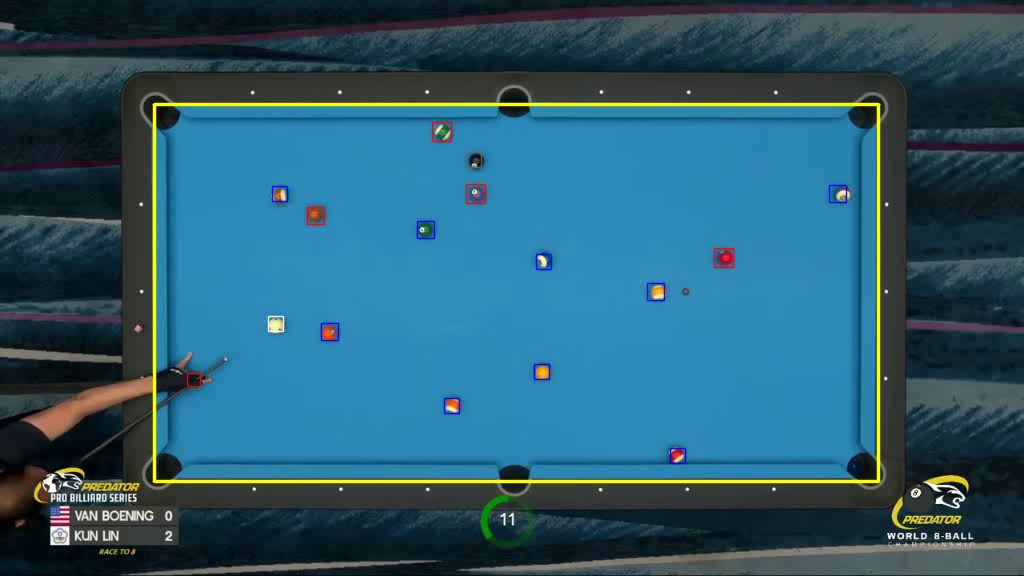
\includegraphics[width=\textwidth]{images/Detection/game1_clip1_detected_balls_first_frame.jpg}
        \caption{Detection game1 clip1 first frame}
        \label{fig: game1_clip1_first_frame_detected}
    \end{subfigure}
    \begin{subfigure}[b]{0.48\textwidth}
        \centering
        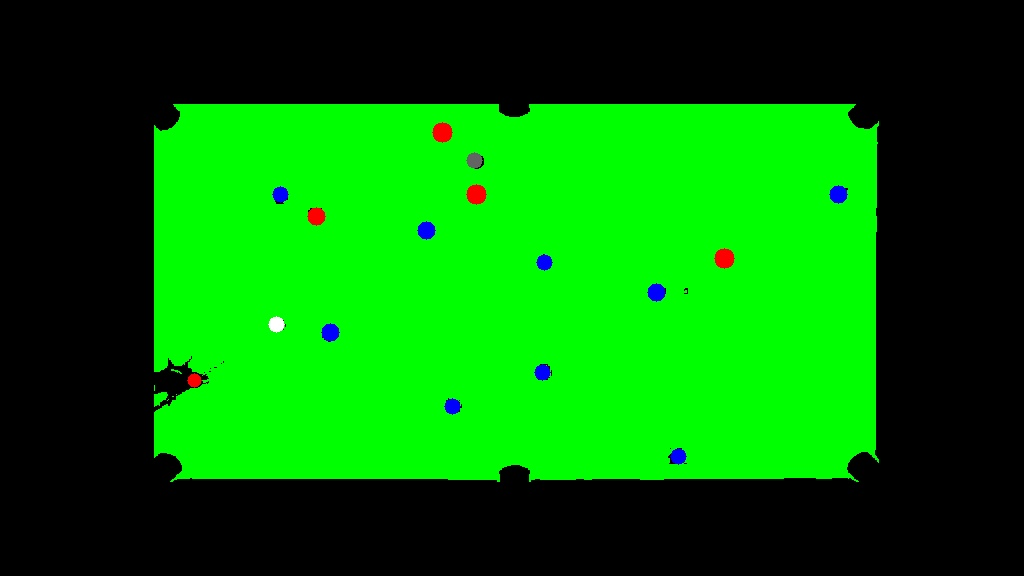
\includegraphics[width=\textwidth]{images/Segmentation/game1_clip1_segmented_balls_first_frame.jpg}
        \caption{Segmentation game1 clip1 first frame}
		\label{fig: game1_clip1_first_frame_segmented}
    \end{subfigure}
    \begin{subfigure}[b]{0.48\textwidth}
        \centering
        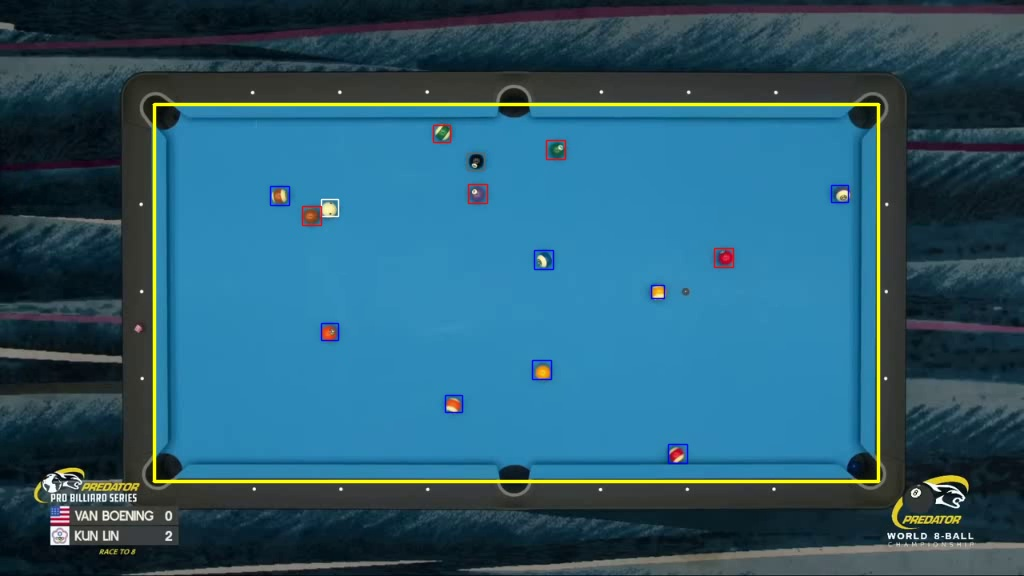
\includegraphics[width=\textwidth]{images/Detection/game1_clip1_detected_balls_last_frame.jpg}
        \caption{Detection game1 clip1 last frame}
        \label{fig: game1_clip1_last_frame_detected}
    \end{subfigure}
    \begin{subfigure}[b]{0.48\textwidth}
        \centering
        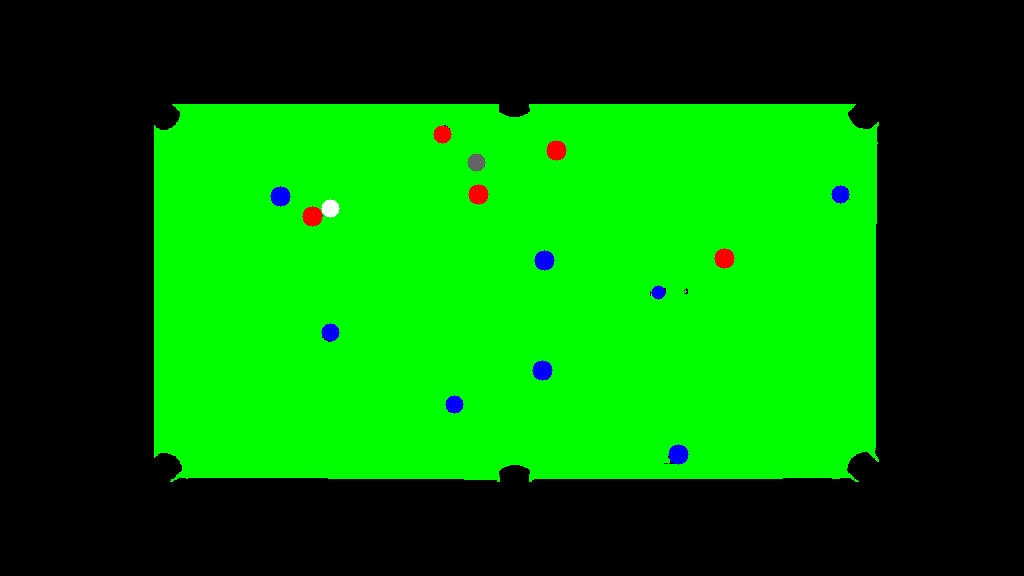
\includegraphics[width=\textwidth]{images/Segmentation/game1_clip1_segmented_balls_last_frame.jpg}
        \caption{Segmentation game1 clip1 last frame}
		\label{fig: game1_clip1_last_frame_segmented}
    \end{subfigure}
    \begin{subfigure}[b]{0.48\textwidth}
    	\centering
    	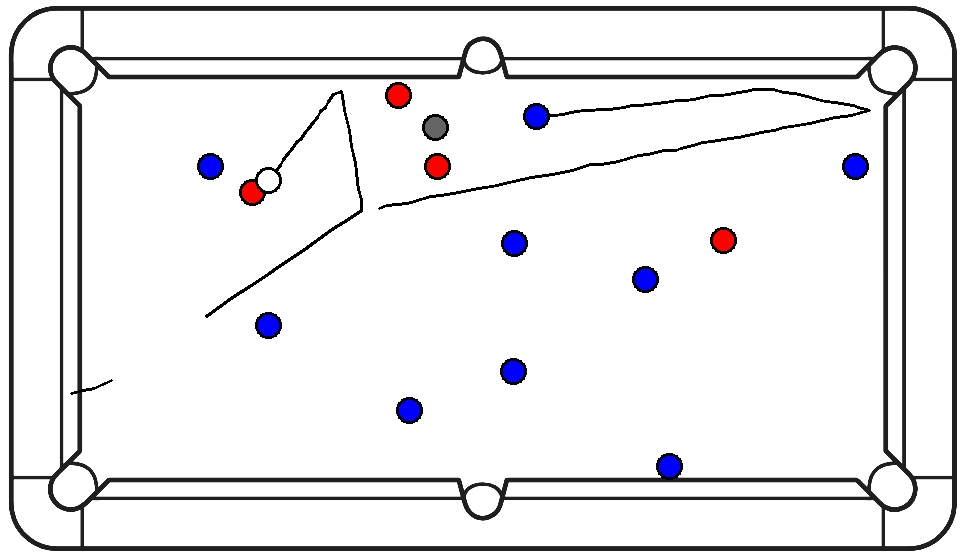
\includegraphics[width=\textwidth]{images/AllMinimap/game1_clip1_minimap.png}
    	\caption{Minimap game1 clip1}
    	\label{fig: game1_clip1_minimap}
    \end{subfigure}
    \begin{subfigure}[b]{0.48\textwidth}
    	\centering
    	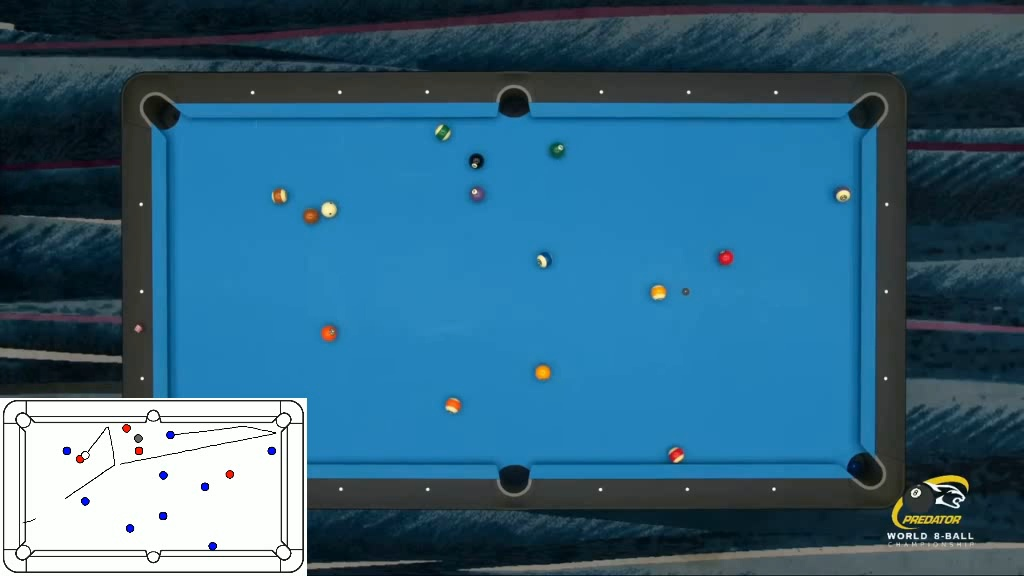
\includegraphics[width=\textwidth]{images/Video/game1_clip1_video.jpg}
    	\caption{Video game1 clip1}
    	\label{fig: game1_clip1_video}
    \end{subfigure}

	\caption{game1 clip1}
\end{figure}

\begin{figure}[H]
    \centering
    \begin{subfigure}[b]{0.48\textwidth}
        \centering
        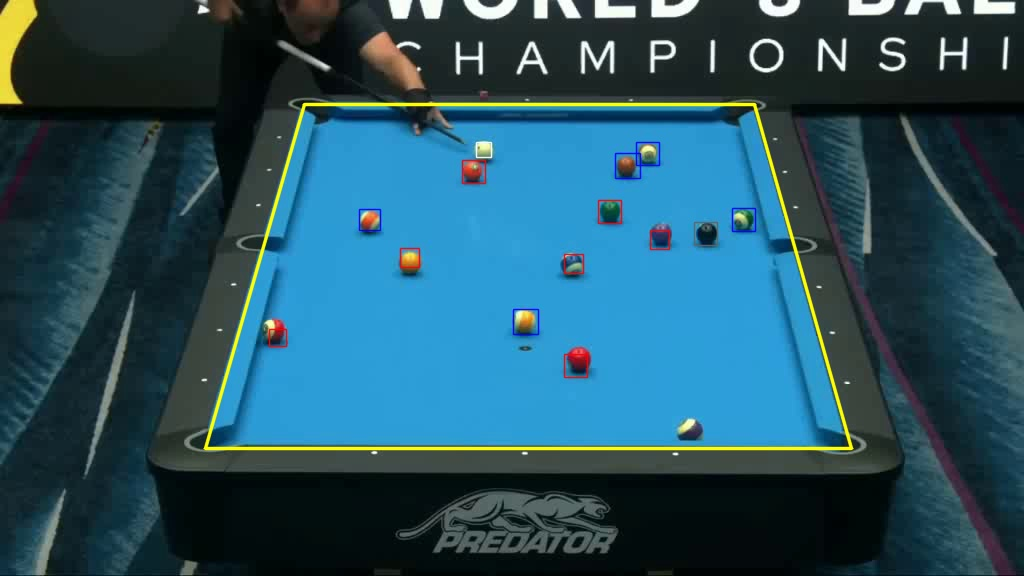
\includegraphics[width=\textwidth]{images/Detection/game1_clip2_detected_balls_first_frame.jpg}
        \caption{Detection game1 clip2 first frame}
        \label{fig: game1_clip2_first_frame_detected}
    \end{subfigure}
    \begin{subfigure}[b]{0.48\textwidth}
        \centering
        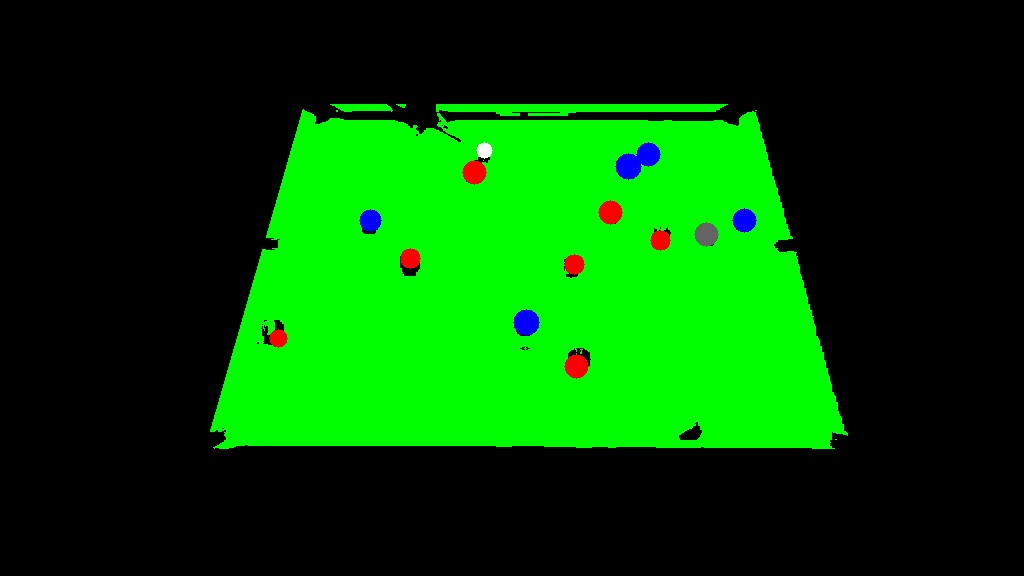
\includegraphics[width=\textwidth]{images/Segmentation/game1_clip2_segmented_balls_first_frame.jpg}
        \caption{Segmentation game1 clip2 first frame}
		\label{fig: game1_clip2_first_frame_segmented}
    \end{subfigure}
    \begin{subfigure}[b]{0.48\textwidth}
        \centering
        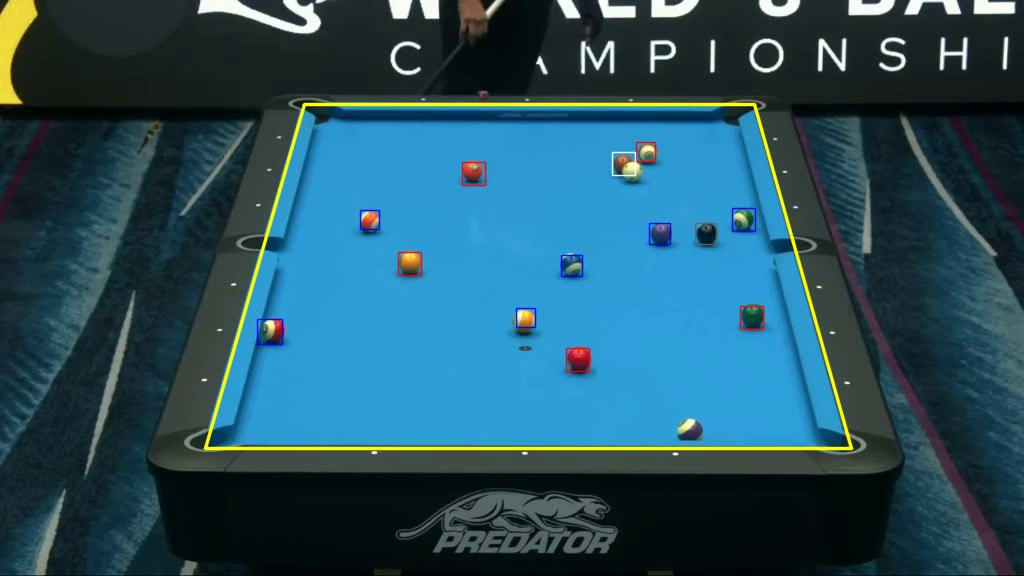
\includegraphics[width=\textwidth]{images/Detection/game1_clip2_detected_balls_last_frame.jpg}
        \caption{Detection game1 clip2 last frame}
        \label{fig: game1_clip2_last_frame_detected}
    \end{subfigure}
    \begin{subfigure}[b]{0.48\textwidth}
        \centering
        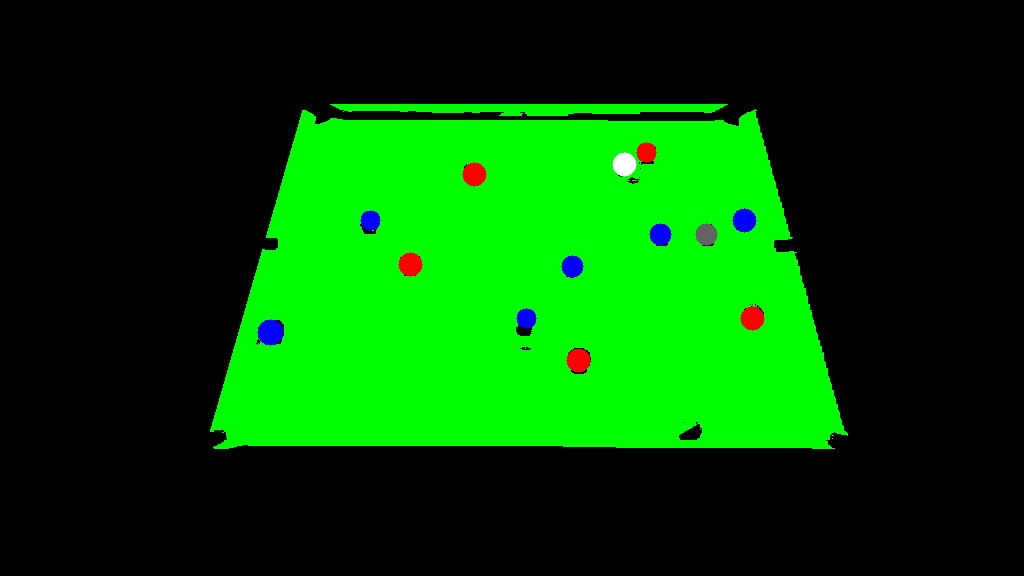
\includegraphics[width=\textwidth]{images/Segmentation/game1_clip2_segmented_balls_last_frame.jpg}
        \caption{Segmentation game1 clip2 last frame}
		\label{fig: game1_clip2_last_frame_segmented}
    \end{subfigure}
    \begin{subfigure}[b]{0.48\textwidth}
    	\centering
    	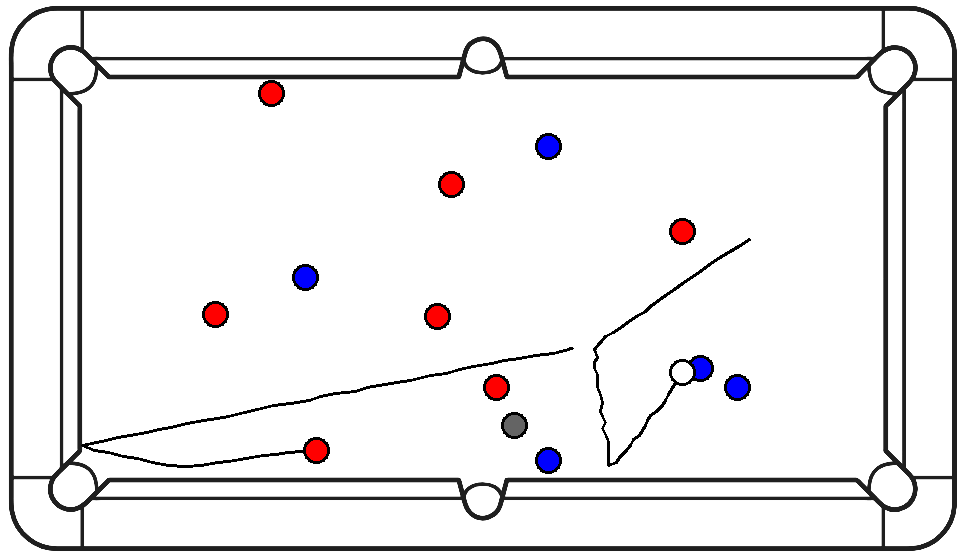
\includegraphics[width=\textwidth]{images/AllMinimap/game1_clip2_minimap.png}
    	\caption{Minimap game1 clip2}
    	\label{fig: game1_clip2_minimap}
    \end{subfigure}
    \begin{subfigure}[b]{0.48\textwidth}
    	\centering
    	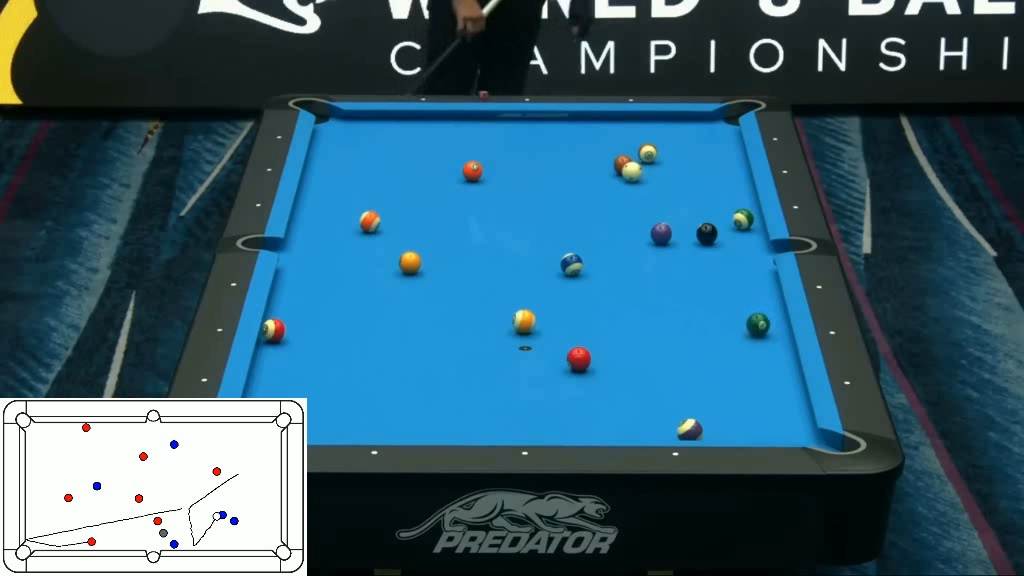
\includegraphics[width=\textwidth]{images/Video/game1_clip2_video.jpg}
    	\caption{Video game1 clip2}
    	\label{fig: game1_clip2_video}
    \end{subfigure}

	\caption{game1 clip2}
\end{figure}

\begin{figure}[H]
    \centering
    \begin{subfigure}[b]{0.48\textwidth}
        \centering
        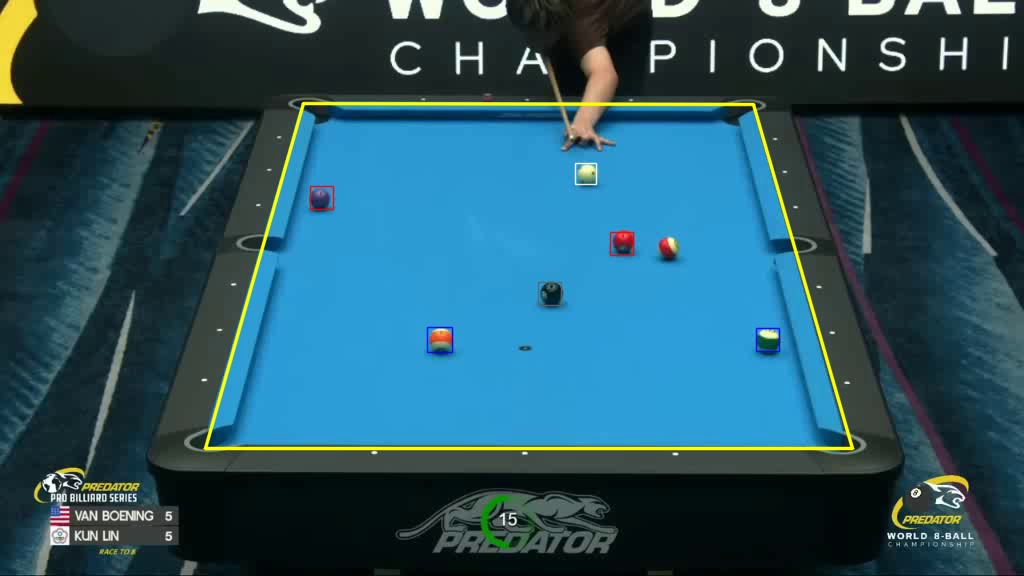
\includegraphics[width=\textwidth]{images/Detection/game1_clip3_detected_balls_first_frame.jpg}
        \caption{Detection game1 clip3 first frame}
        \label{fig: game1_clip3_first_frame_detected}
    \end{subfigure}
    \begin{subfigure}[b]{0.48\textwidth}
        \centering
        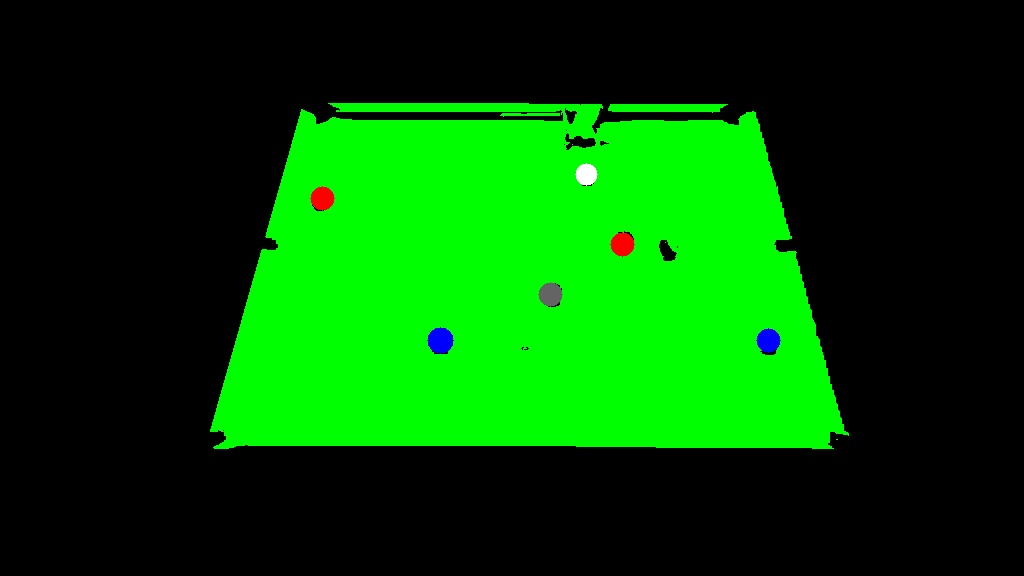
\includegraphics[width=\textwidth]{images/Segmentation/game1_clip3_segmented_balls_first_frame.jpg}
        \caption{Segmentation game1 clip3 first frame}
		\label{fig: game1_clip3_first_frame_segmented}
    \end{subfigure}
    \begin{subfigure}[b]{0.48\textwidth}
        \centering
        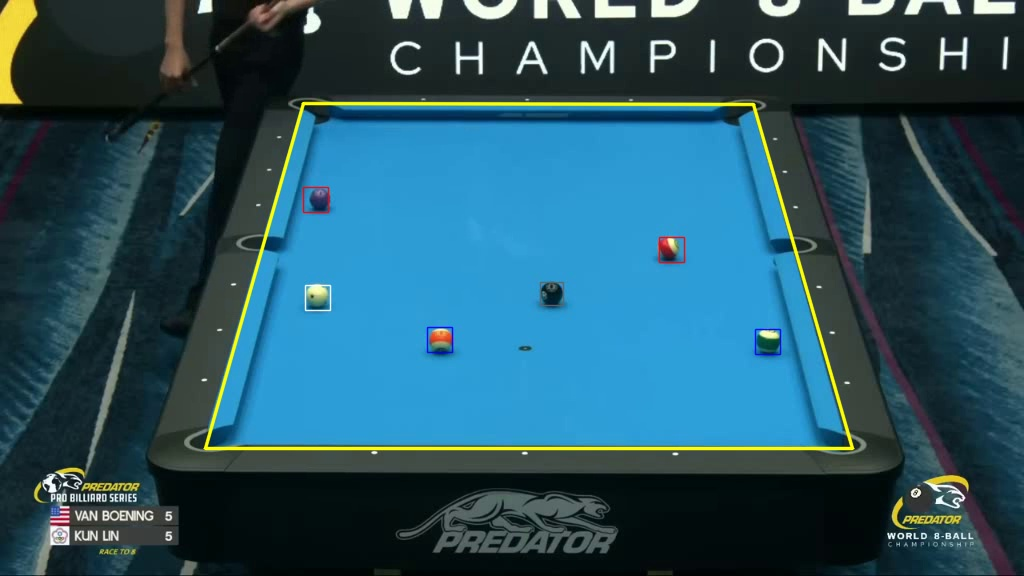
\includegraphics[width=\textwidth]{images/Detection/game1_clip3_detected_balls_last_frame.jpg}
        \caption{Detection game1 clip3 last frame}
        \label{fig: game1_clip3_last_frame_detected}
    \end{subfigure}
    \begin{subfigure}[b]{0.48\textwidth}
        \centering
        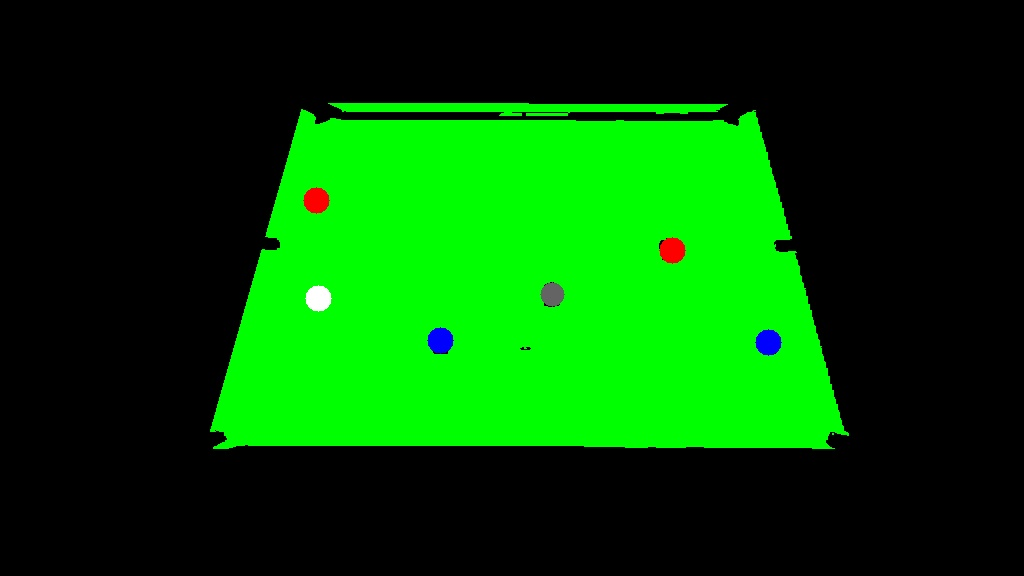
\includegraphics[width=\textwidth]{images/Segmentation/game1_clip3_segmented_balls_last_frame.jpg}
        \caption{Segmentation game1 clip3 last frame}
		\label{fig: game1_clip3_last_frame_segmented}
    \end{subfigure}
    \begin{subfigure}[b]{0.48\textwidth}
    	\centering
    	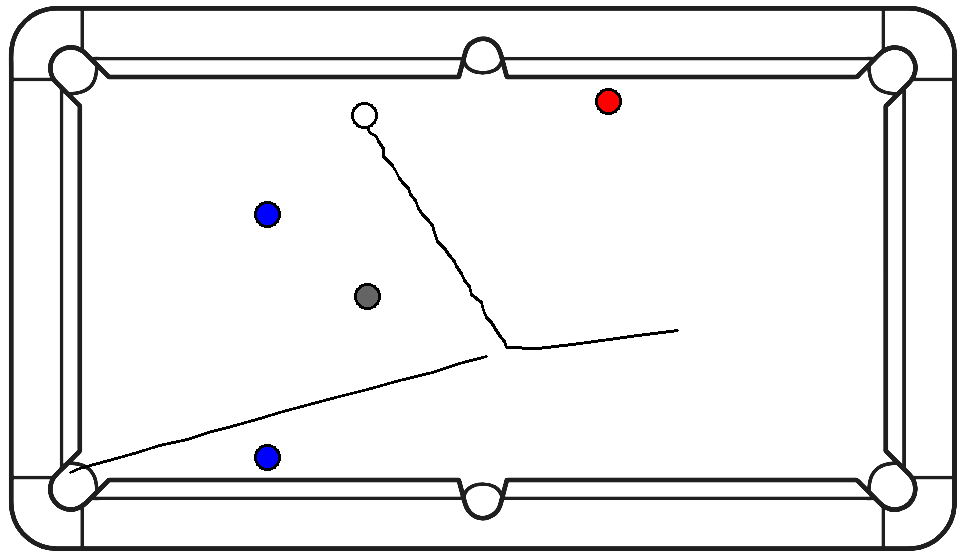
\includegraphics[width=\textwidth]{images/AllMinimap/game1_clip3_minimap.png}
    	\caption{Minimap game1 clip3}
    	\label{fig: game1_clip3_minimap}
    \end{subfigure}
    \begin{subfigure}[b]{0.48\textwidth}
    	\centering
    	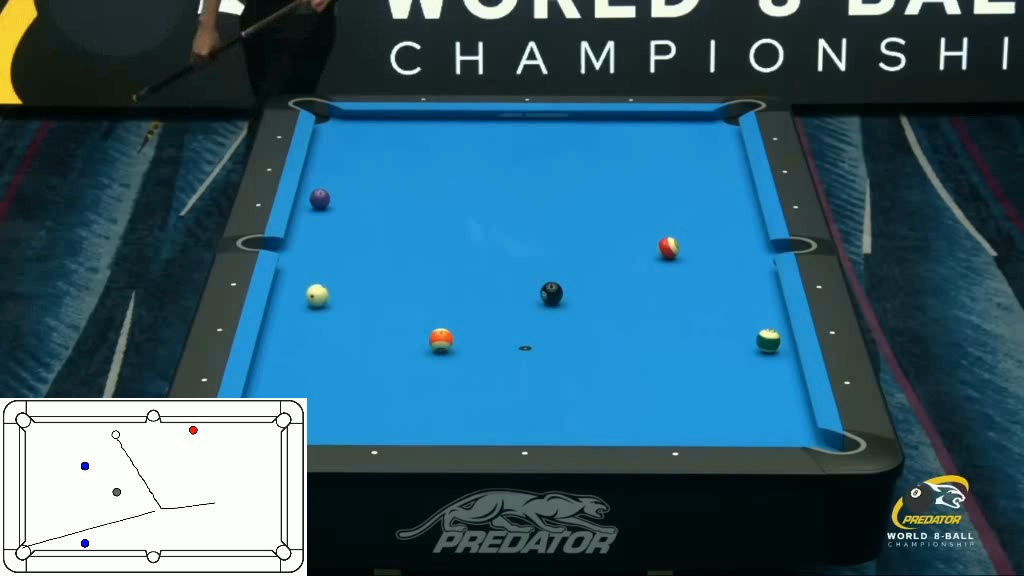
\includegraphics[width=\textwidth]{images/Video/game1_clip3_video.jpg}
    	\caption{Video game1 clip3}
    	\label{fig: game1_clip3_video}
    \end{subfigure}

	\caption{game1 clip3}
\end{figure}

\begin{figure}[H]
    \centering
    \begin{subfigure}[b]{0.48\textwidth}
        \centering
        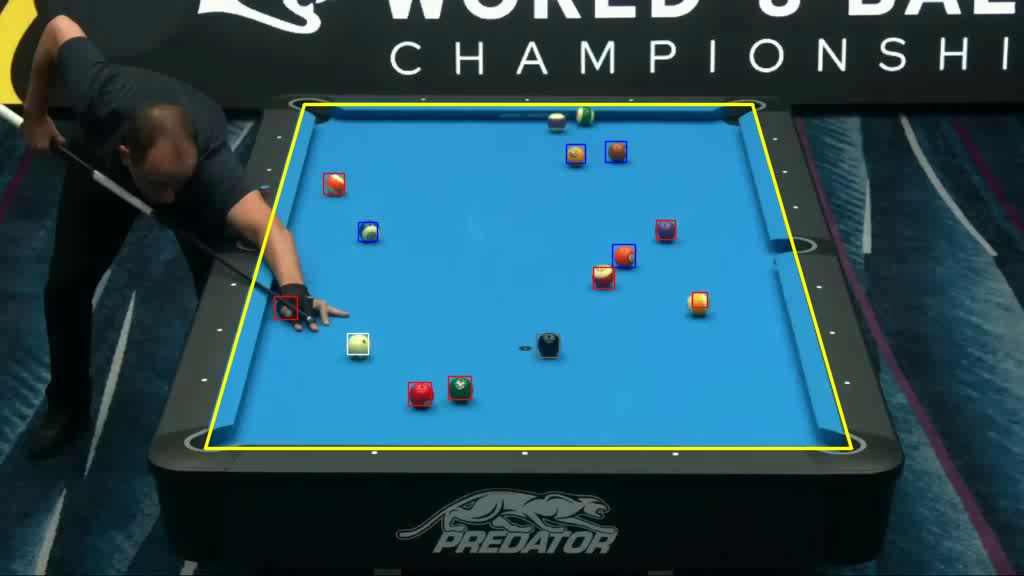
\includegraphics[width=\textwidth]{images/Detection/game1_clip4_detected_balls_first_frame.jpg}
        \caption{Detection game1 clip4 first frame}
        \label{fig: game1_clip4_first_frame_detected}
    \end{subfigure}
    \begin{subfigure}[b]{0.48\textwidth}
        \centering
        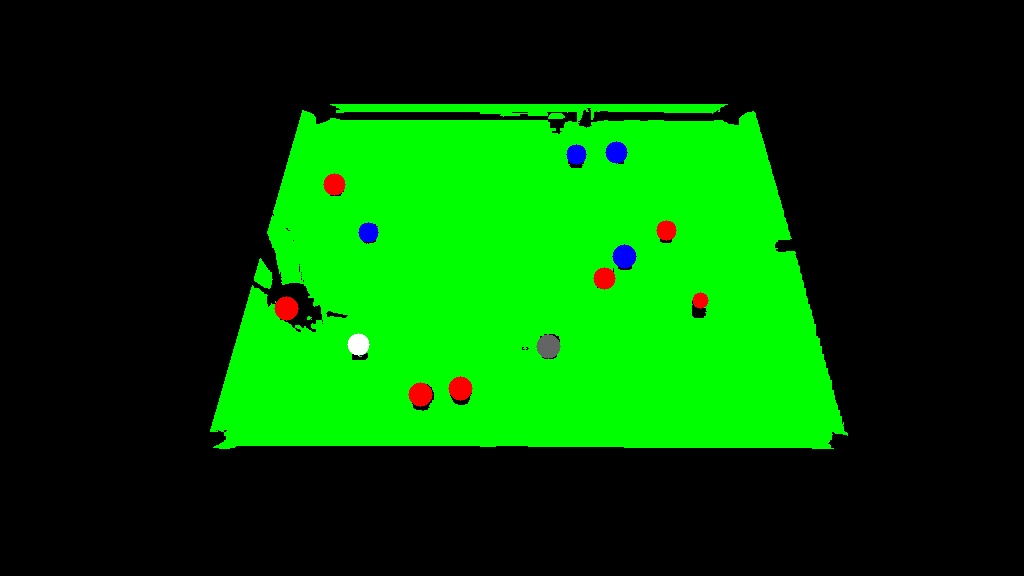
\includegraphics[width=\textwidth]{images/Segmentation/game1_clip4_segmented_balls_first_frame.jpg}
        \caption{Segmentation game1 clip4 first frame}
		\label{fig: game1_clip4_first_frame_segmented}
    \end{subfigure}
    \begin{subfigure}[b]{0.48\textwidth}
        \centering
        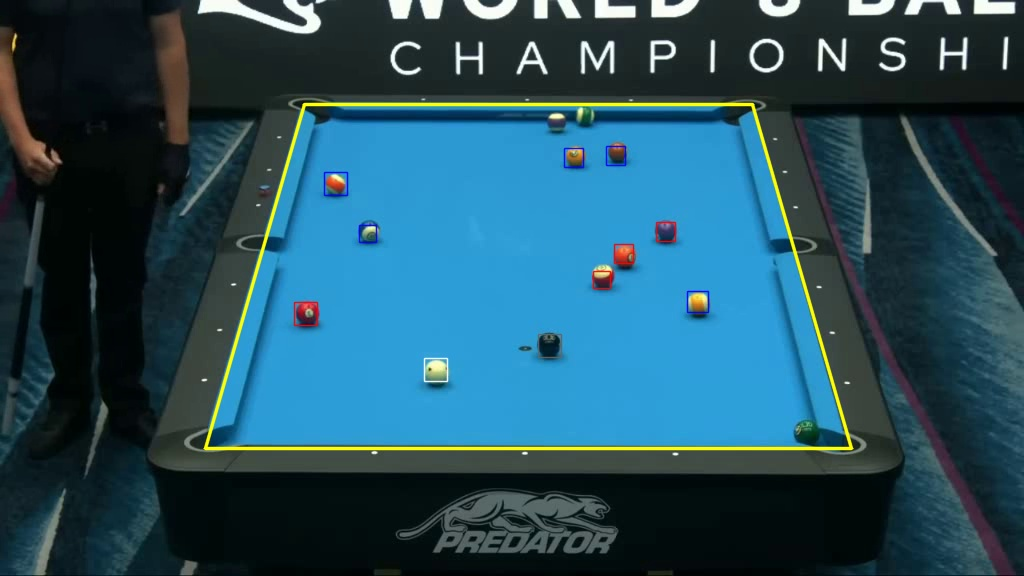
\includegraphics[width=\textwidth]{images/Detection/game1_clip4_detected_balls_last_frame.jpg}
        \caption{Detection game1 clip4 last frame}
        \label{fig: game1_clip4_last_frame_detected}
    \end{subfigure}
    \begin{subfigure}[b]{0.48\textwidth}
        \centering
        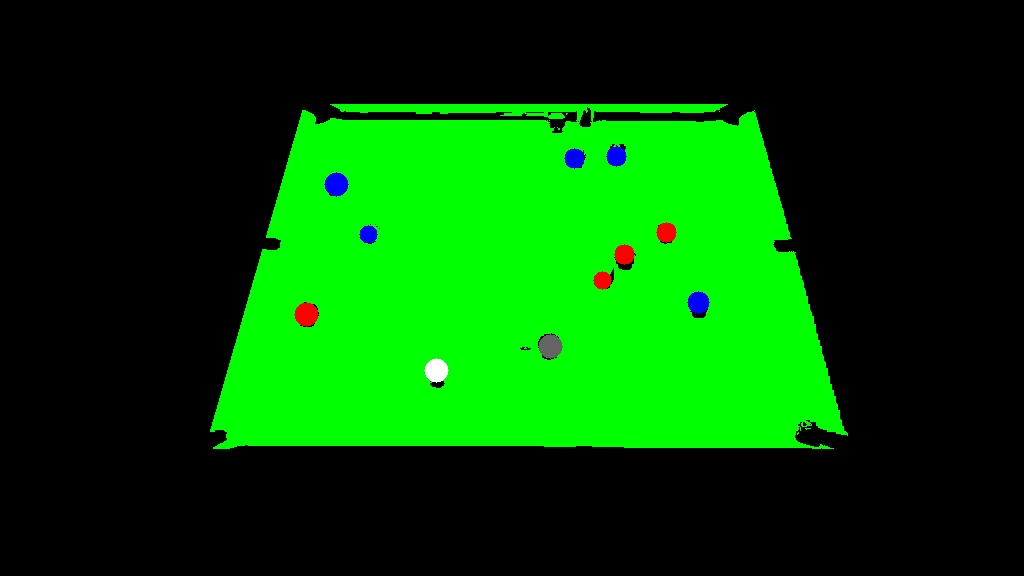
\includegraphics[width=\textwidth]{images/Segmentation/game1_clip4_segmented_balls_last_frame.jpg}
        \caption{Segmentation game1 clip4 last frame}
		\label{fig: game1_clip4_last_frame_segmented}
    \end{subfigure}
    \begin{subfigure}[b]{0.48\textwidth}
    	\centering
    	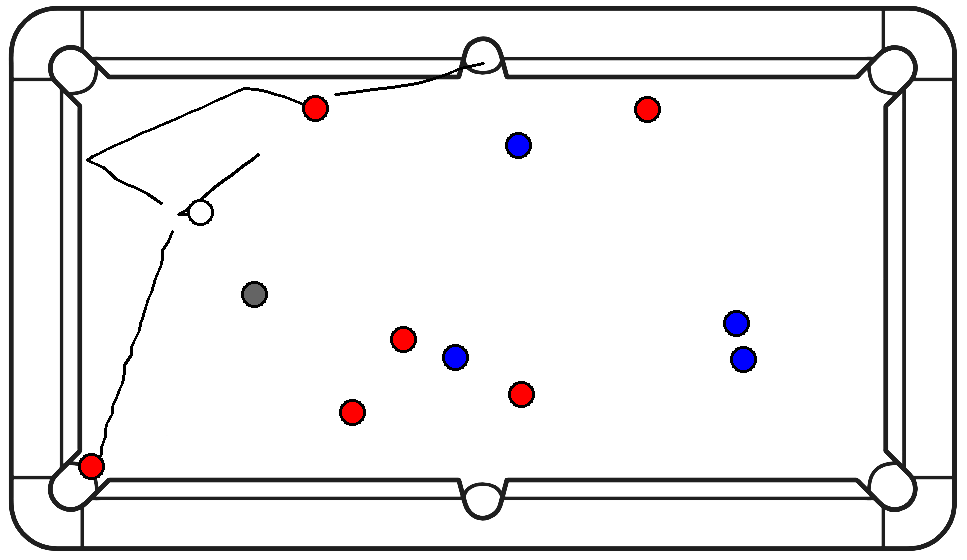
\includegraphics[width=\textwidth]{images/AllMinimap/game1_clip4_minimap.png}
    	\caption{Minimap game1 clip4}
    	\label{fig: game1_clip4_minimap}
    \end{subfigure}
    \begin{subfigure}[b]{0.48\textwidth}
    	\centering
    	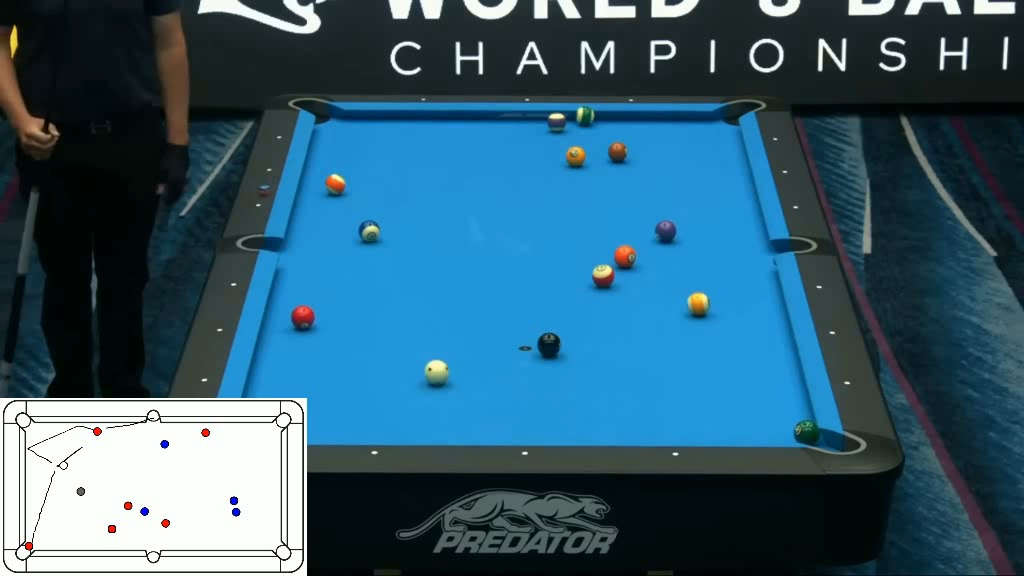
\includegraphics[width=\textwidth]{images/Video/game1_clip4_video.jpg}
    	\caption{Video game1 clip4}
    	\label{fig: game1_clip4_video}
    \end{subfigure}

	\caption{game1 clip4}
\end{figure}


\begin{figure}[H]
    \centering
    \begin{subfigure}[b]{0.48\textwidth}
        \centering
        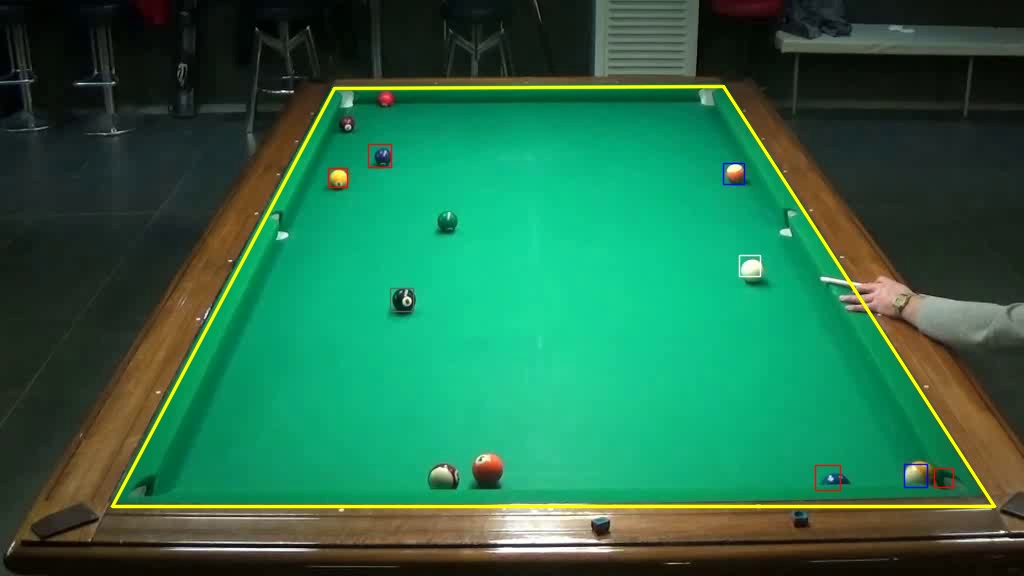
\includegraphics[width=\textwidth]{images/Detection/game2_clip1_detected_balls_first_frame.jpg}
        \caption{Detection game2 clip1 first frame}
        \label{fig: game2_clip1_first_frame_detected}
    \end{subfigure}
    \begin{subfigure}[b]{0.48\textwidth}
        \centering
        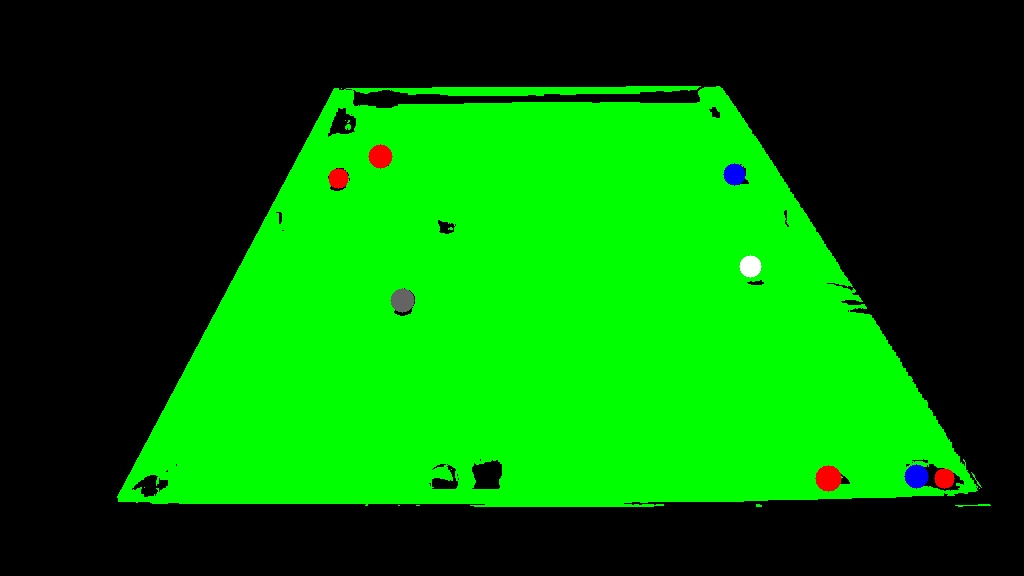
\includegraphics[width=\textwidth]{images/Segmentation/game2_clip1_segmented_balls_first_frame.jpg}
        \caption{Segmentation game2 clip1 first frame}
		\label{fig: game2_clip1_first_frame_segmented}
    \end{subfigure}
    \centering
    \begin{subfigure}[b]{0.48\textwidth}
        \centering
        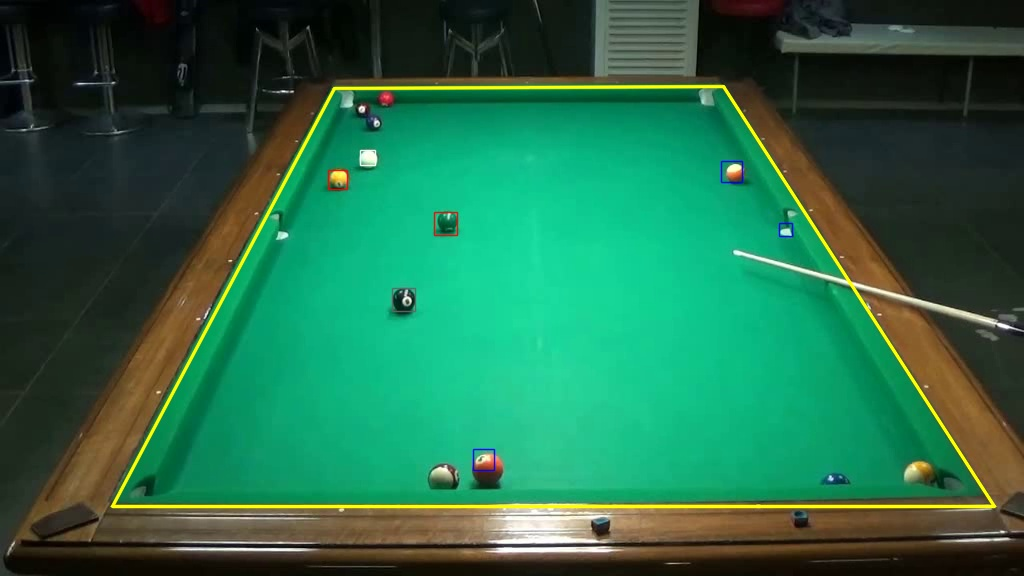
\includegraphics[width=\textwidth]{images/Detection/game2_clip1_detected_balls_last_frame.jpg}
        \caption{Detection game2 clip1 last frame}
        \label{fig: game2_clip1_last_frame_detected}
    \end{subfigure}
    \begin{subfigure}[b]{0.48\textwidth}
        \centering
        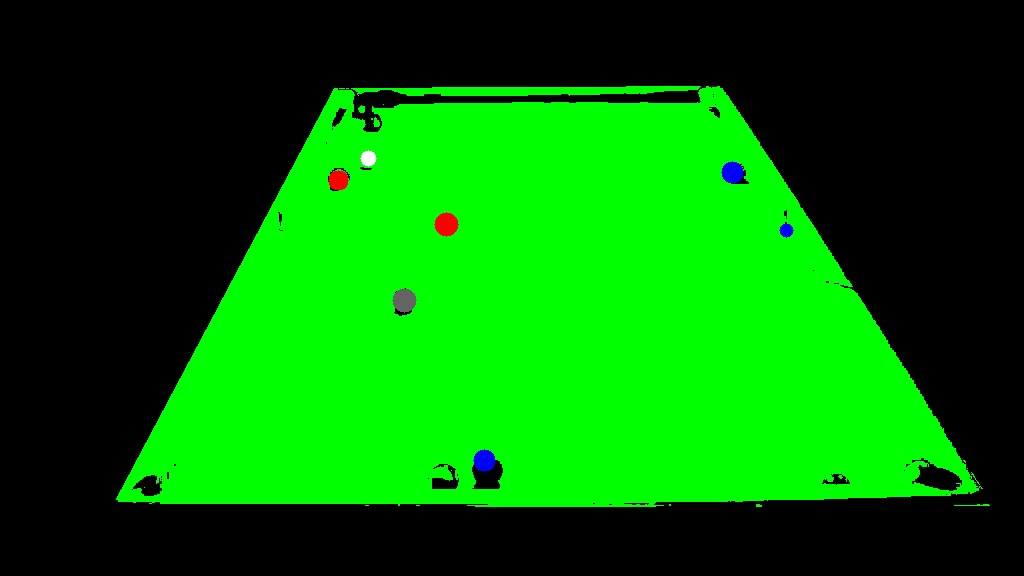
\includegraphics[width=\textwidth]{images/Segmentation/game2_clip1_segmented_balls_last_frame.jpg}
        \caption{Segmentation game2 clip1 last frame}
		\label{fig: game2_clip1_last_frame_segmented}
    \end{subfigure}
    \begin{subfigure}[b]{0.48\textwidth}
    	\centering
    	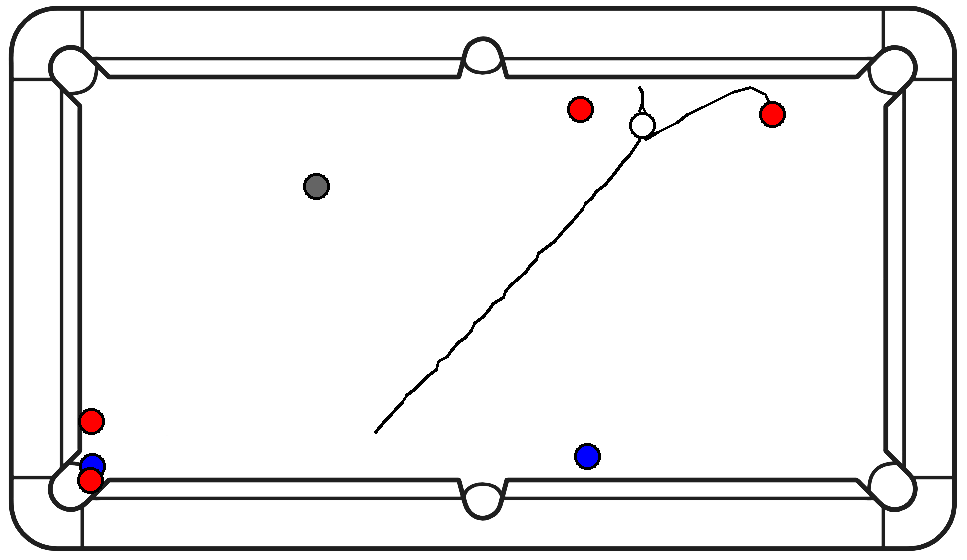
\includegraphics[width=\textwidth]{images/AllMinimap/game2_clip1_minimap.png}
    	\caption{Minimap game2 clip1}
    	\label{fig: game2_clip1_minimap}
    \end{subfigure}
    \begin{subfigure}[b]{0.48\textwidth}
    	\centering
    	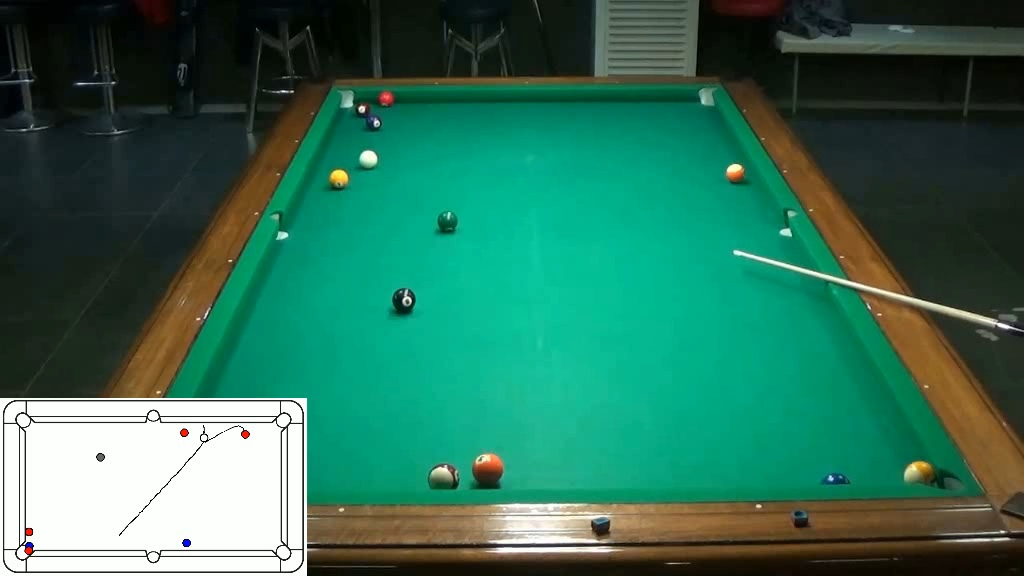
\includegraphics[width=\textwidth]{images/Video/game2_clip1_video.jpg}
    	\caption{Video game2 clip1}
    	\label{fig: game2_clip1_video}
    \end{subfigure}

	\caption{game2 clip1}
\end{figure}


\begin{figure}[H]
    \centering
    \begin{subfigure}[b]{0.48\textwidth}
        \centering
        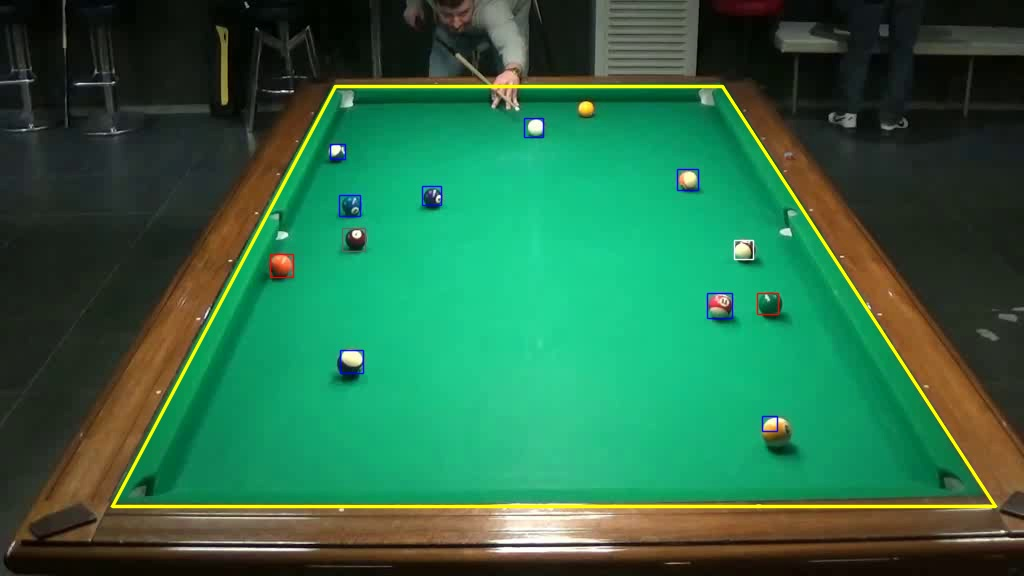
\includegraphics[width=\textwidth]{images/Detection/game2_clip2_detected_balls_first_frame.jpg}
        \caption{Detection game2 clip2 first frame}
        \label{fig: game2_clip2_first_frame_detected}
    \end{subfigure}
    \begin{subfigure}[b]{0.48\textwidth}
        \centering
        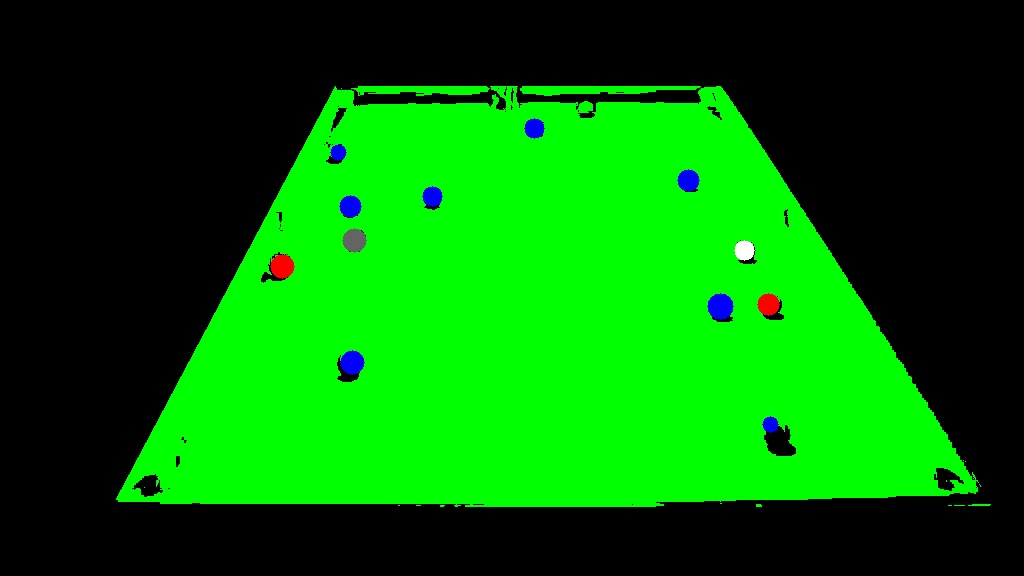
\includegraphics[width=\textwidth]{images/Segmentation/game2_clip2_segmented_balls_first_frame.jpg}
        \caption{Segmentation game2 clip2 first frame}
		\label{fig: game2_clip2_first_frame_segmented}
    \end{subfigure}
    \begin{subfigure}[b]{0.48\textwidth}
        \centering
        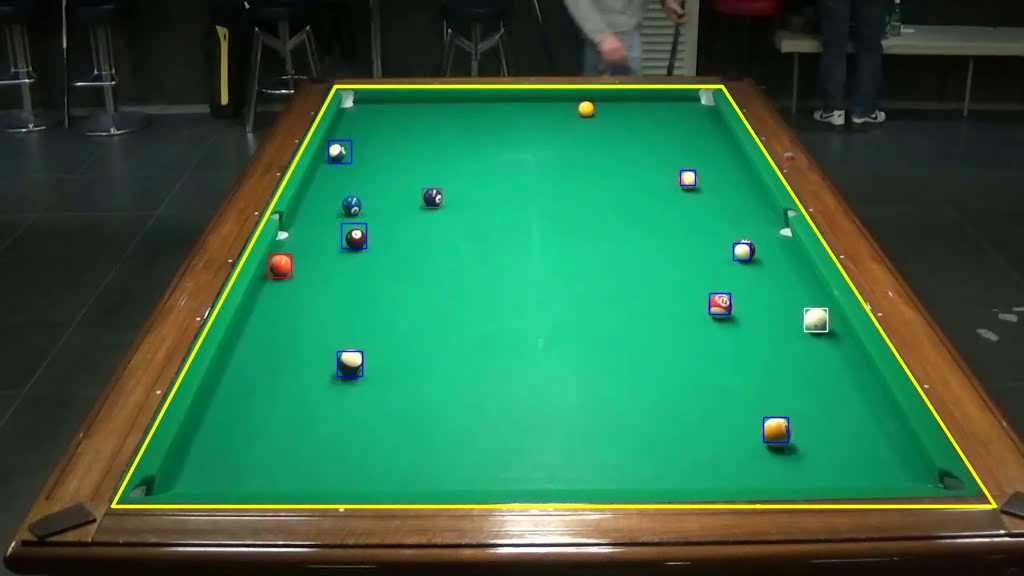
\includegraphics[width=\textwidth]{images/Detection/game2_clip2_detected_balls_last_frame.jpg}
        \caption{Detection game2 clip2 last frame}
        \label{fig: game2_clip2_last_frame_detected}
    \end{subfigure}
    \begin{subfigure}[b]{0.48\textwidth}
        \centering
        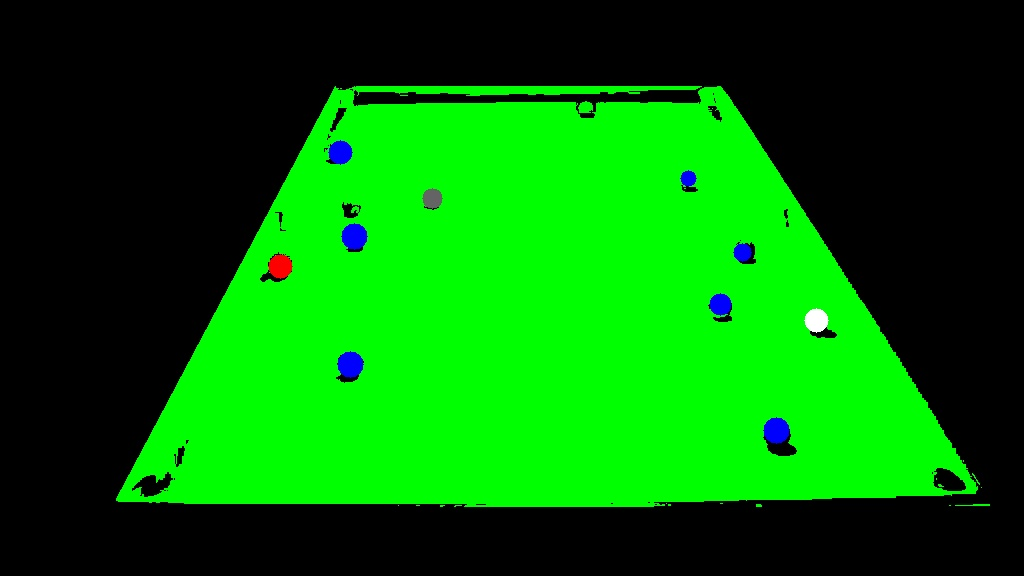
\includegraphics[width=\textwidth]{images/Segmentation/game2_clip2_segmented_balls_last_frame.jpg}
        \caption{Segmentation game2 clip2 last frame}
		\label{fig: game2_clip2_last_frame_segmented}
    \end{subfigure}
    \begin{subfigure}[b]{0.48\textwidth}
    	\centering
    	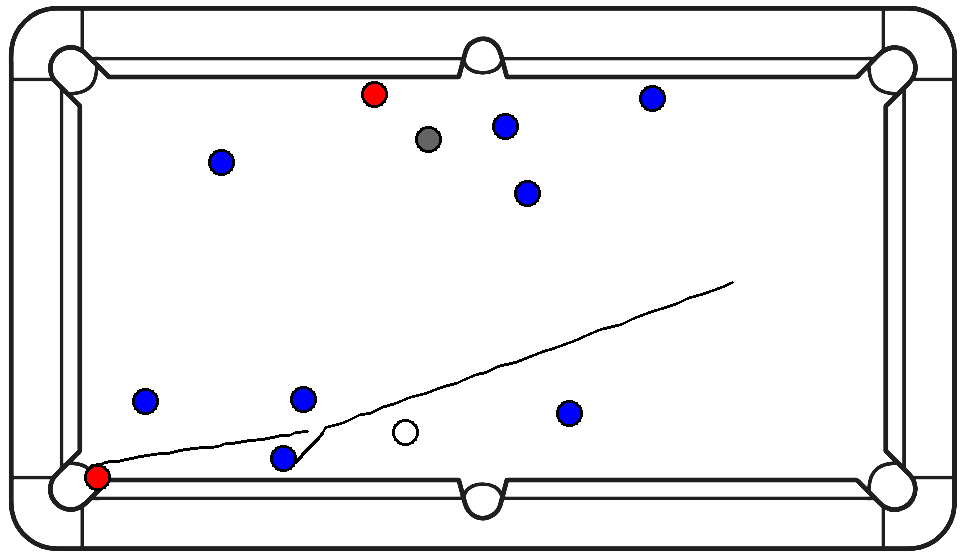
\includegraphics[width=\textwidth]{images/AllMinimap/game2_clip2_minimap.png}
    	\caption{Minimap game2 clip2}
    	\label{fig: game2_clip2_minimap}
    \end{subfigure}
    \begin{subfigure}[b]{0.48\textwidth}
    	\centering
    	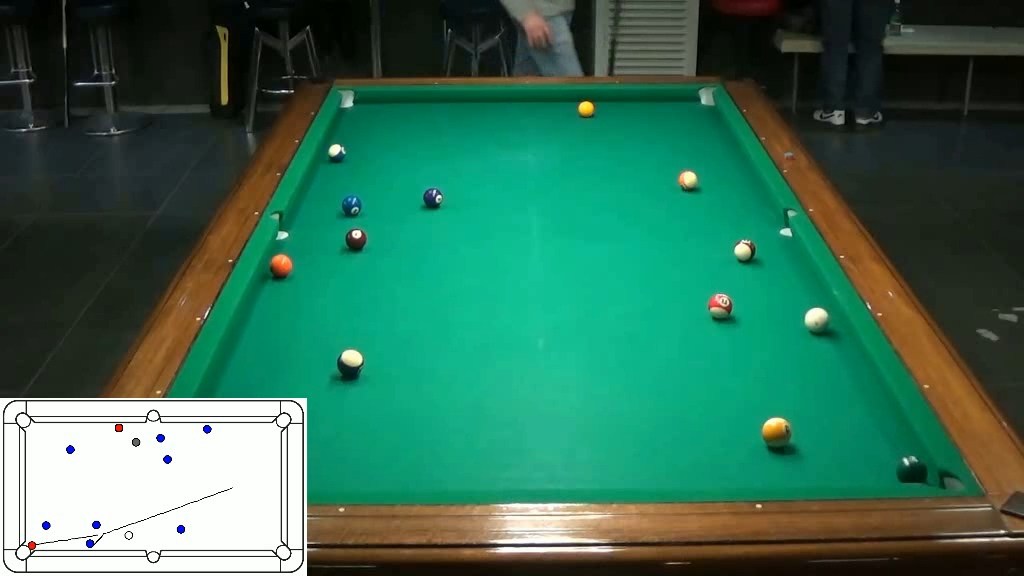
\includegraphics[width=\textwidth]{images/Video/game2_clip2_video.jpg}
    	\caption{Video game2 clip2}
    	\label{fig: game2_clip2_video}
    \end{subfigure}

	\caption{game2 clip2}
\end{figure}

\begin{figure}[H]
    \centering
    \begin{subfigure}[b]{0.48\textwidth}
        \centering
        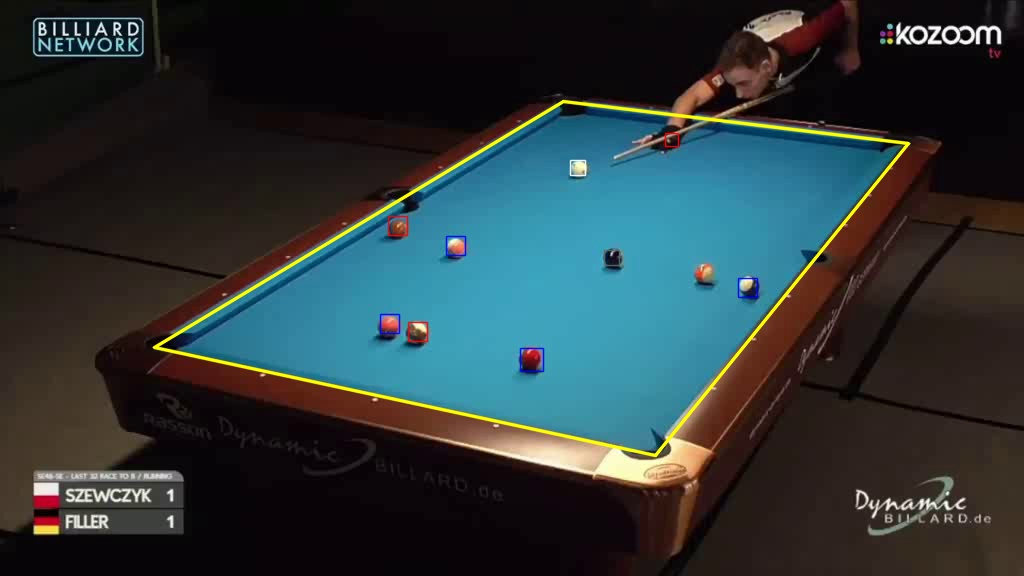
\includegraphics[width=\textwidth]{images/Detection/game3_clip1_detected_balls_first_frame.jpg}
        \caption{Detection game3 clip1 first frame}
        \label{fig: game3_clip1_first_frame_detected}
    \end{subfigure}
    \begin{subfigure}[b]{0.48\textwidth}
        \centering
        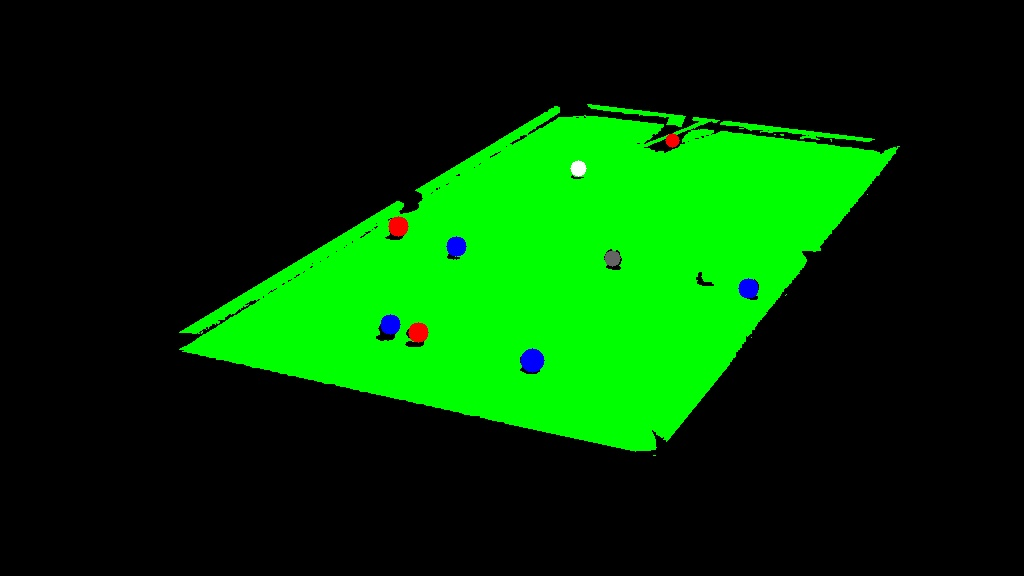
\includegraphics[width=\textwidth]{images/Segmentation/game3_clip1_segmented_balls_first_frame.jpg}
        \caption{Segmentation game3 clip1 first frame}
		\label{fig: game3_clip1_first_frame_segmented}
    \end{subfigure}
    \begin{subfigure}[b]{0.48\textwidth}
        \centering
        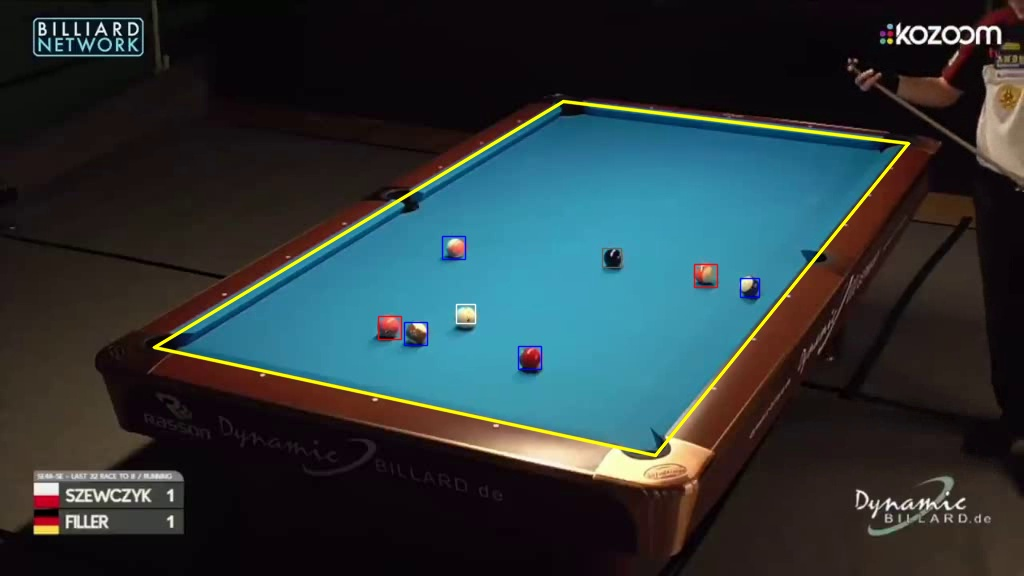
\includegraphics[width=\textwidth]{images/Detection/game3_clip1_detected_balls_last_frame.jpg}
        \caption{Detection game3 clip1 last frame}
        \label{fig: game3_clip1_last_frame_detected}
    \end{subfigure}
    \begin{subfigure}[b]{0.48\textwidth}
        \centering
        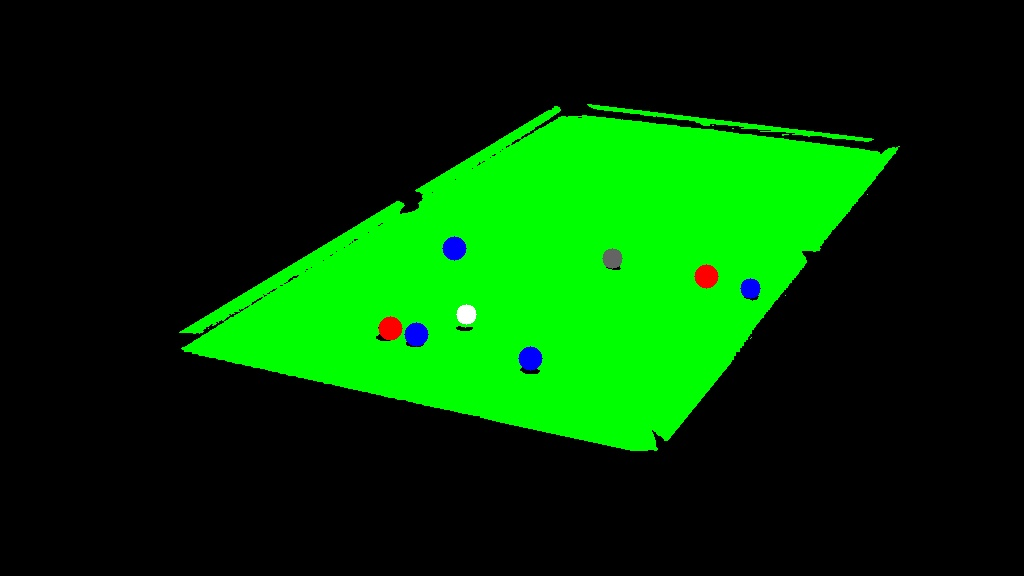
\includegraphics[width=\textwidth]{images/Segmentation/game3_clip1_segmented_balls_last_frame.jpg}
        \caption{Segmentation game3 clip1 last frame}
		\label{fig: game3_clip1_last_frame_segmented}
    \end{subfigure}
    \begin{subfigure}[b]{0.48\textwidth}
    	\centering
    	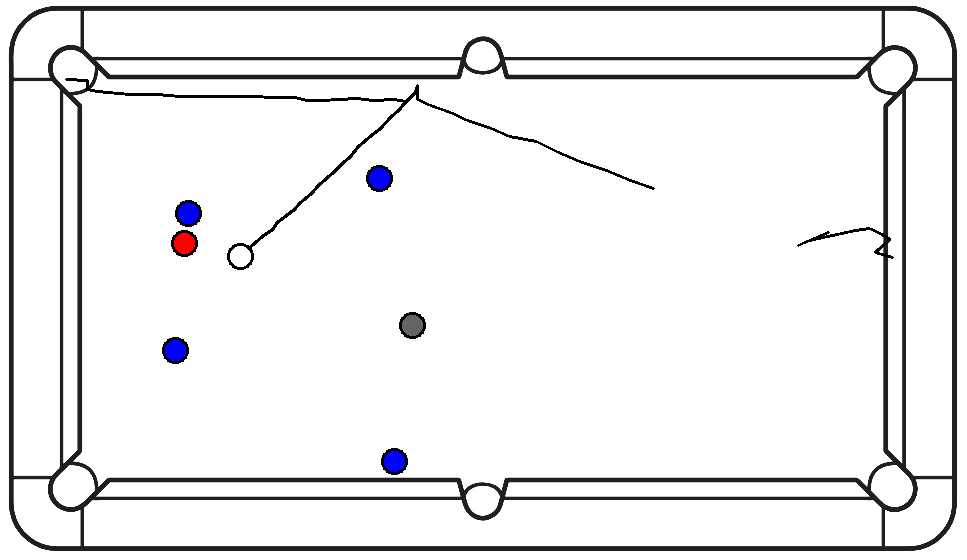
\includegraphics[width=\textwidth]{images/AllMinimap/game3_clip1_minimap.png}
    	\caption{Minimap game3 clip1}
    	\label{fig: game3_clip1_minimap}
    \end{subfigure}
    \begin{subfigure}[b]{0.48\textwidth}
    	\centering
    	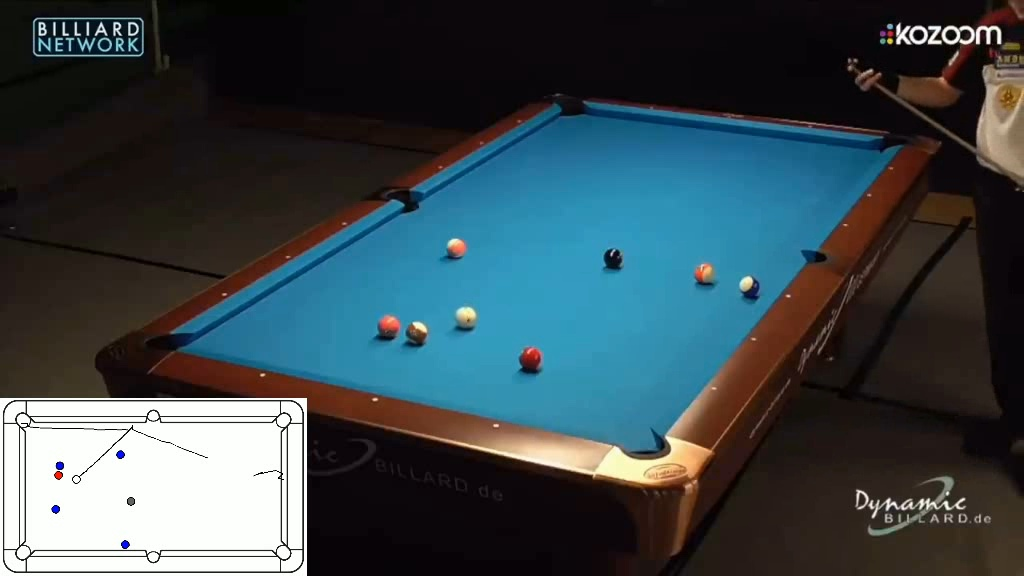
\includegraphics[width=\textwidth]{images/Video/game3_clip1_video.jpg}
    	\caption{Video game3 clip1}
    	\label{fig: game3_clip1_video}
    \end{subfigure}

	\caption{game3 clip1}
\end{figure}

\begin{figure}[H]
    \centering
    \begin{subfigure}[b]{0.48\textwidth}
        \centering
        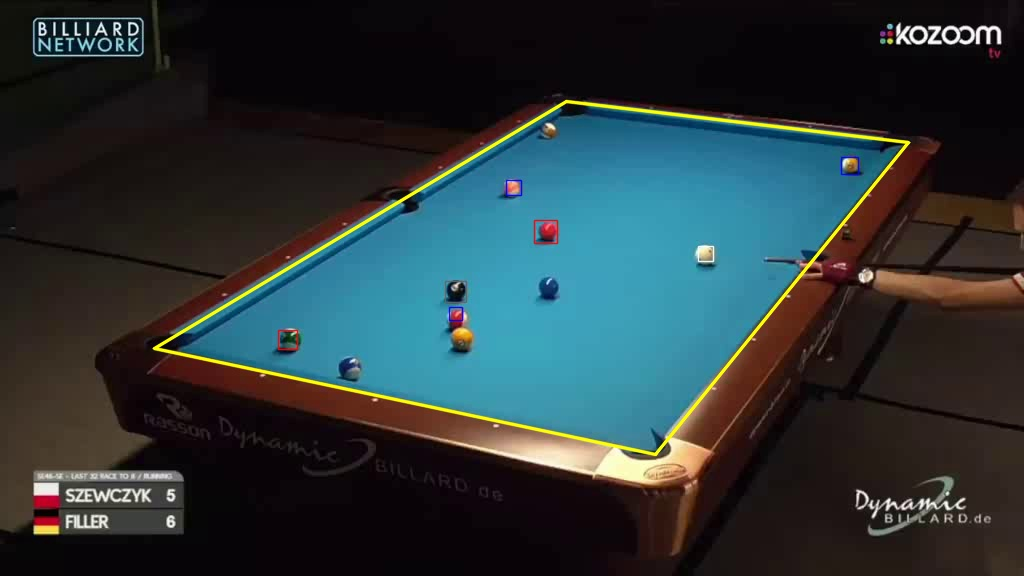
\includegraphics[width=\textwidth]{images/Detection/game3_clip2_detected_balls_first_frame.jpg}
        \caption{Detection game3 clip2 first frame}
        \label{fig: game3_clip2_first_frame_detected}
    \end{subfigure}
    \begin{subfigure}[b]{0.48\textwidth}
        \centering
        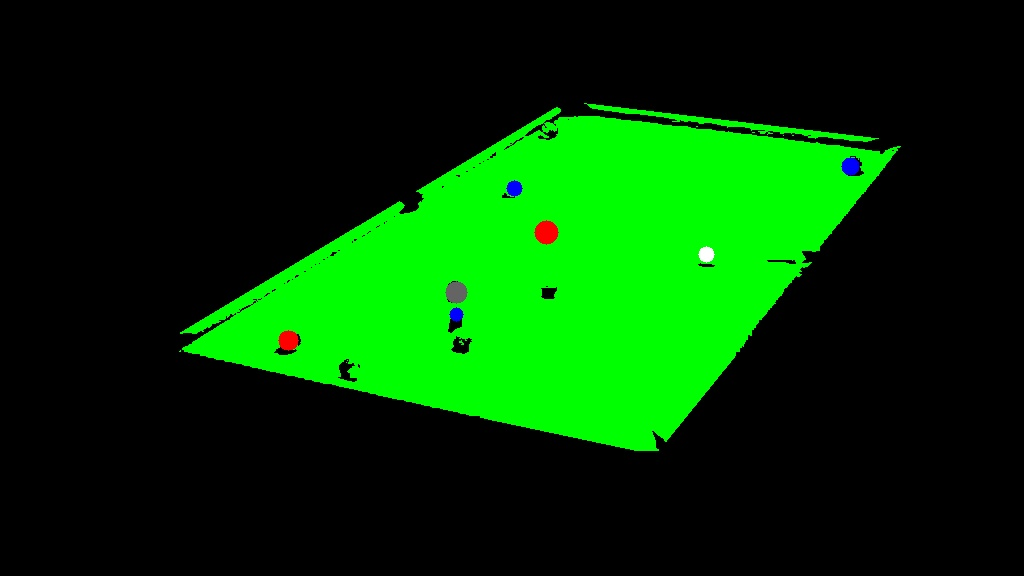
\includegraphics[width=\textwidth]{images/Segmentation/game3_clip2_segmented_balls_first_frame.jpg}
        \caption{Segmentation game3 clip2 first frame}
		\label{fig: game3_clip2_first_frame_segmented}
    \end{subfigure}
    \begin{subfigure}[b]{0.48\textwidth}
        \centering
        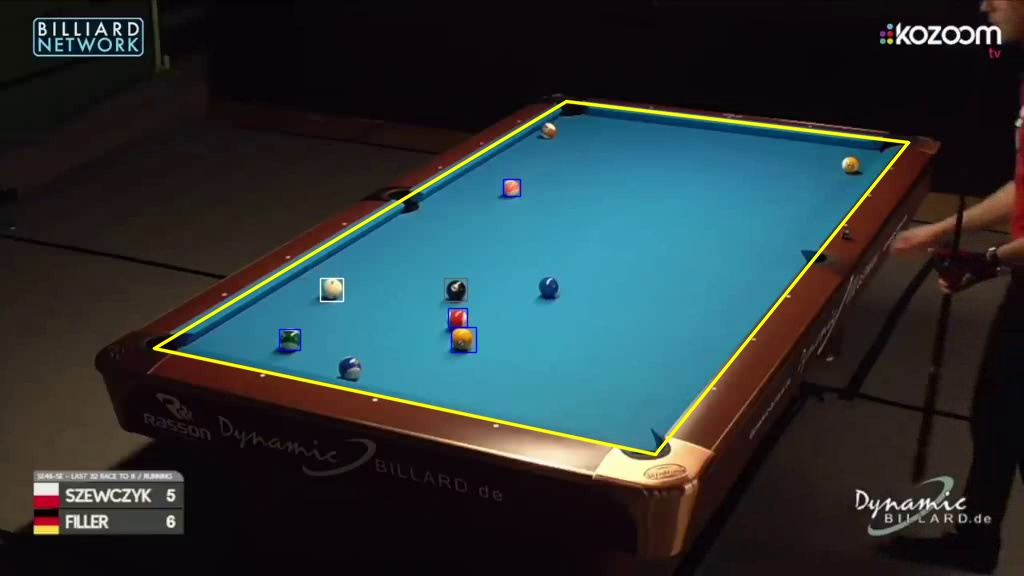
\includegraphics[width=\textwidth]{images/Detection/game3_clip2_detected_balls_last_frame.jpg}
        \caption{Detection game3 clip2 last frame}
        \label{fig: game3_clip2_last_frame_detected}
    \end{subfigure}
    \begin{subfigure}[b]{0.48\textwidth}
        \centering
        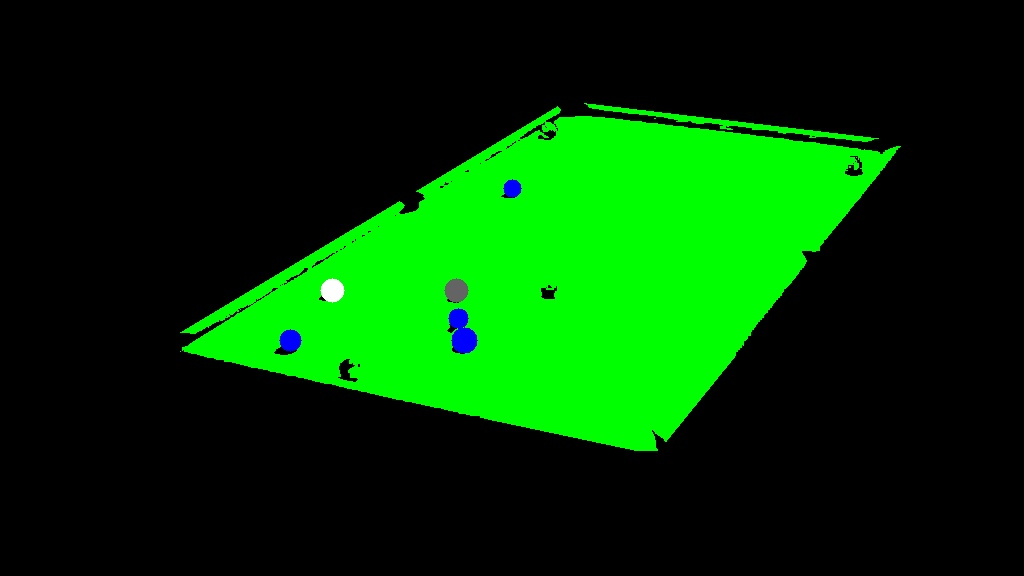
\includegraphics[width=\textwidth]{images/Segmentation/game3_clip2_segmented_balls_last_frame.jpg}
        \caption{Segmentation game3 clip2 last frame}
		\label{fig: game3_clip2_last_frame_segmented}
    \end{subfigure}
    \begin{subfigure}[b]{0.48\textwidth}
    	\centering
    	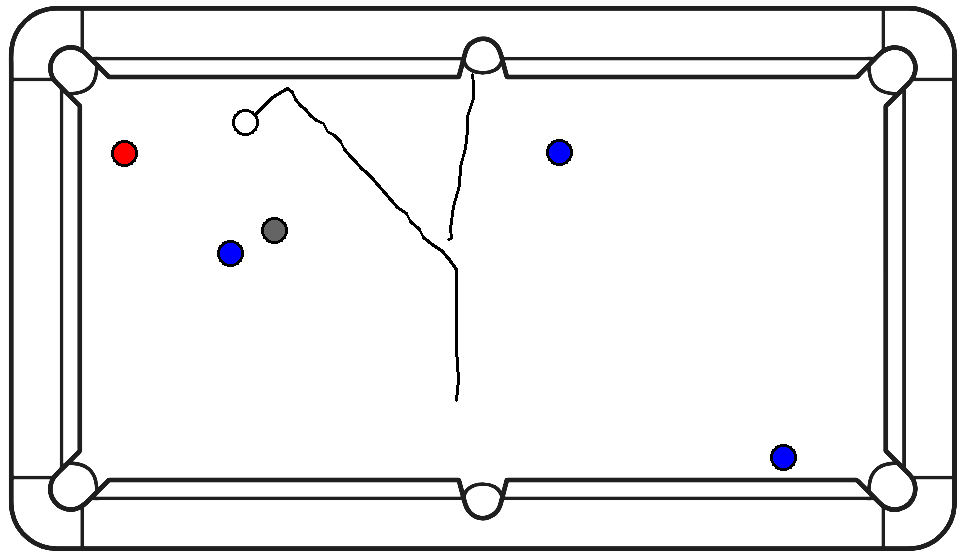
\includegraphics[width=\textwidth]{images/AllMinimap/game3_clip2_minimap.png}
    	\caption{Minimap game3 clip2}
    	\label{fig: game3_clip2_minimap}
    \end{subfigure}
    \begin{subfigure}[b]{0.48\textwidth}
    	\centering
    	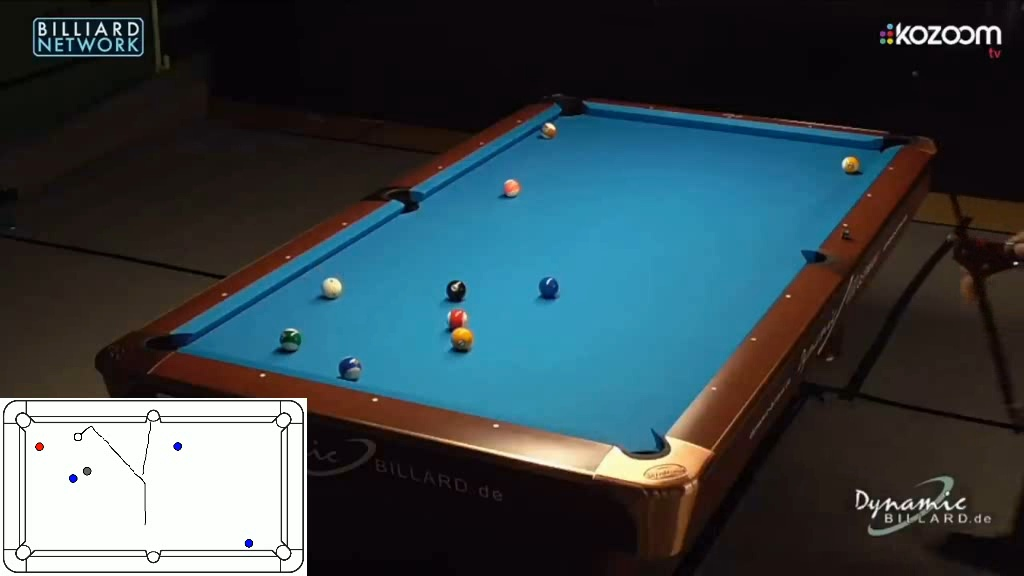
\includegraphics[width=\textwidth]{images/Video/game3_clip2_video.jpg}
    	\caption{Video game3 clip2}
    	\label{fig: game3_clip2_video}
    \end{subfigure}

	\caption{game3 clip2}
\end{figure}

\begin{figure}[H]
    \centering
    \begin{subfigure}[b]{0.48\textwidth}
        \centering
        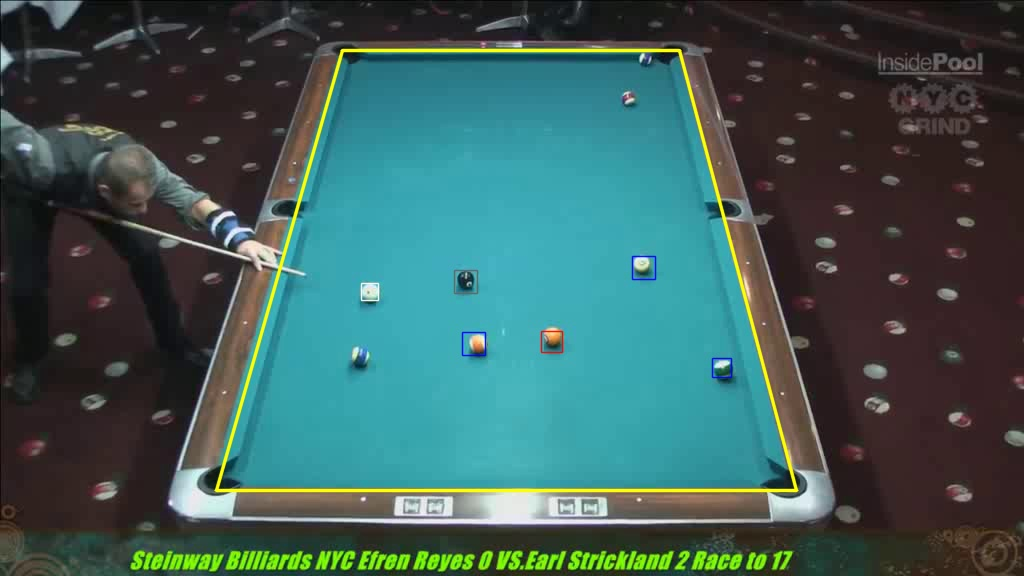
\includegraphics[width=\textwidth]{images/Detection/game4_clip1_detected_balls_first_frame.jpg}
        \caption{Detection game4 clip1 first frame}
        \label{fig: game4_clip1_first_frame_detected}
    \end{subfigure}
    \begin{subfigure}[b]{0.48\textwidth}
        \centering
        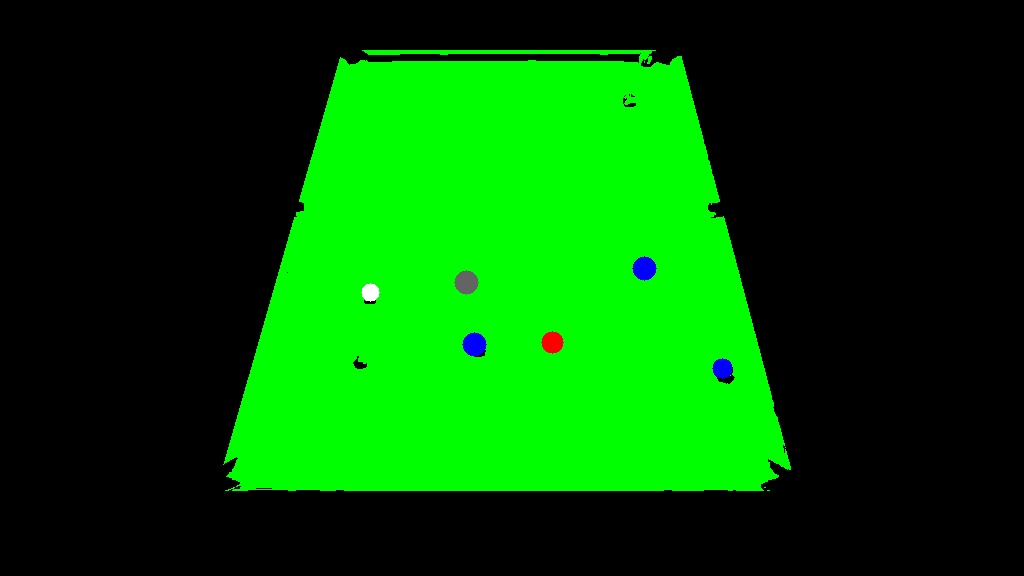
\includegraphics[width=\textwidth]{images/Segmentation/game4_clip1_segmented_balls_first_frame.jpg}
        \caption{Segmentation game4 clip1 first frame}
		\label{fig: game4_clip1_first_frame_segmented}
    \end{subfigure}
    \begin{subfigure}[b]{0.48\textwidth}
        \centering
        \includegraphics[width=\textwidth]{images/Detection/game4_clip1_detected_balls_last_frame.jpg}
        \caption{Detection game4 clip1 last frame}
        \label{fig: game4_clip1_last_frame_detected}
    \end{subfigure}
    \begin{subfigure}[b]{0.48\textwidth}
        \centering
        \includegraphics[width=\textwidth]{images/Segmentation/game4_clip1_segmented_balls_last_frame.jpg}
        \caption{Segmentation game4 clip1 last frame}
		\label{fig: game4_clip1_last_frame_segmented}
    \end{subfigure}
    \begin{subfigure}[b]{0.48\textwidth}
    	\centering
    	\includegraphics[width=\textwidth]{images/AllMinimap/game4_clip1_minimap.png}
    	\caption{Minimap game4 clip1}
    	\label{fig: game4_clip1_minimap}
    \end{subfigure}
    \begin{subfigure}[b]{0.48\textwidth}
    	\centering
    	\includegraphics[width=\textwidth]{images/Video/game4_clip1_video.jpg}
    	\caption{Video game4 clip1}
    	\label{fig: game4_clip1_video}
    \end{subfigure}

	\caption{game4 clip1}
\end{figure}


\begin{figure}[H]
    \centering
    \begin{subfigure}[b]{0.48\textwidth}
        \centering
        \includegraphics[width=\textwidth]{images/Detection/game4_clip2_detected_balls_first_frame.jpg}
        \caption{Detection game4 clip2 first frame}
        \label{fig: game4_clip2_first_frame_detected}
    \end{subfigure}
    \begin{subfigure}[b]{0.48\textwidth}
        \centering
        \includegraphics[width=\textwidth]{images/Segmentation/game4_clip2_segmented_balls_first_frame.jpg}
        \caption{Segmentation game4 clip2 first frame}
		\label{fig: game4_clip2_first_frame_segmented}
    \end{subfigure}
    \begin{subfigure}[b]{0.48\textwidth}
        \centering
        \includegraphics[width=\textwidth]{images/Detection/game4_clip2_detected_balls_last_frame.jpg}
        \caption{Detection game4 clip2 last frame}
        \label{fig: game4_clip2_last_frame_detected}
    \end{subfigure}
    \begin{subfigure}[b]{0.48\textwidth}
        \centering
        \includegraphics[width=\textwidth]{images/Segmentation/game4_clip2_segmented_balls_last_frame.jpg}
        \caption{Segmentation game4 clip2 last frame}
		\label{fig: game4_clip2_last_frame_segmented}
    \end{subfigure}
    \begin{subfigure}[b]{0.48\textwidth}
    	\centering
    	\includegraphics[width=\textwidth]{images/AllMinimap/game4_clip2_minimap.png}
    	\caption{Minimap game4 clip2}
    	\label{fig: game4_clip2_minimap}
    \end{subfigure}
    \begin{subfigure}[b]{0.48\textwidth}
    	\centering
    	\includegraphics[width=\textwidth]{images/Video/game4_clip2_video.jpg}
    	\caption{Video game4 clip2}
    	\label{fig: game1_clip1_video}
    \end{subfigure}

	\caption{game4 clip2}
\end{figure}


\subsection{Quantitative results}
The \textit{computePerformance} executable calculates the detection and segmentation performance across the dataset.
\begin{table}[H]
	\centering
    \begin{tabular}{|c|c|}
        \hline
        \textbf{Class} & \textbf{AP} \\
        \hline
        white & 0.90 \\
        \hline
        black & 0.44 \\
        \hline
        solid & 0.31 \\
        \hline
        striped & 0.38 \\
        \hline
    \end{tabular}
    \caption{AP of the detection across the dataset}
    \label{tab: AP across dataset}
\end{table}

\begin{table}[H]
	\centering
    \begin{tabular}{|c|c|}
        \hline
        \textbf{Class} & \textbf{IoU} \\
        \hline
        background & 0.97 \\
        \hline
        white & 0.67 \\
        \hline
        black & 0.75 \\
        \hline
        solid & 0.36 \\
        \hline
        striped & 0.39 \\
        \hline
        playing field & 0.95 \\
        \hline
    \end{tabular}
    \caption{IoU of the detection across the dataset}
    \label{tab: IoU across dataset}
\end{table}

\begin{table}[H]
	\centering
    \begin{tabular}{|c|c|}
        \hline
        \textbf{mAP} & \textbf{mIoU} \\
        \hline
        0.51 & 0.69 \\
        \hline
    \end{tabular}
    \caption{Performance of the detection and segmentation across the dataset}
    \label{tab: performance across dataset}
\end{table}
While the method successfully detects tables, backgrounds, and both white and black balls with high Intersection
over Union (IoU), it struggles with solid and striped balls due to inaccurate classification.
This leads to a lower overall mean Average Precision (mAP) that is focused only on balls,
but a good mean Intersection over Union (mIoU) because the background and playing field are identified well.
